%; whizzy chapter
% -initex iniptex -latex platex -format platex -bibtex jbibtex -fmt fmt
% 以上 whizzytex を使用する場合の設定。

%     Tokyo Debian Meeting resources
%     Copyright (C) 2011 Junichi Uekawa
%     Copyright (C) 2011 Nobuhiro Iwamatsu
%     Copyright (C) 2012 Koichi Akabe

%     This program is free software; you can redistribute it and/or modify
%     it under the terms of the GNU General Public License as published by
%     the Free Software Foundation; either version 2 of the License, or
%     (at your option) any later version.

%     This program is distributed in the hope that it will be useful,
%     but WITHOUT ANY WARRANTY; without even the implied warranty of
%     MERCHANTABILITY or FITNESS FOR A PARTICULAR PURPOSE.  See the
%     GNU General Public License for more details.

%     You should have received a copy of the GNU General Public License
%     along with this program; if not, write to the Free Software
%     Foundation, Inc., 51 Franklin St, Fifth Floor, Boston, MA  02110-1301 USA

%  preview (shell-command (concat "evince " (replace-regexp-in-string "tex$" "pdf"(buffer-file-name)) "&"))
% 画像ファイルを処理するためにはebbを利用してboundingboxを作成。
%(shell-command "cd image201201; ebb *.png")

%%ここからヘッダ開始。

\documentclass[mingoth,a4paper]{jsarticle}
\usepackage{monthlyreport}
\usepackage{subfigure}
\renewcommand*\thesubfigure{}

% 日付を定義する、毎月変わります。
\newcommand{\debmtgyear}{2012}
\newcommand{\debmtgmonth}{6}
\newcommand{\debmtgdate}{23}
% (+ (* (- 2012 2005) 12) 12 -1) started from zero
\newcommand{\debmtgnumber}{95}


\begin{document}


%------------------------------------------------------------------------------
\dancersection{TeXLive2011(2012/dev) in Debian}{佐々木洋平}
\label{sec:TeXLive2011}
%------------------------------------------------------------------------------

\subsection{はじめに}

発表要旨を
「Debianにおける{\TeX}環境(特に日本語処理)の導入や設定
および次期安定版Wheezyでの変更点および開発状況について解説します。」
としたので、その順番で解説してみます。
%
ちなみに佐々木はあくまで {\TeX}({\pLaTeX}) のユーザであって、
開発に関してはあまり関与しておりません。
%
また「{\TeX}でナベアツ」とか「{\TeX}で数値計算」とか
そういう話はしませんので、あらかじめご了承下さい。

\subsection{{\TeX}環境(特に日本語処理)って?}
\label{subsec:history}


先ずは「{\TeX}環境、特に日本語処理」について簡単に触れておきます。
%
{\TeX}はDonald E. Knuthさんによって作成された組版(くみはん)システムであり、現在のバージョン番号は 3.1415926 です\footnote{%
  Knuth先生は1990年に{\TeX}の開発終了を宣言しており、
  今後は変更は行なわれません。
  バグフィックスなどでバージョン番号を変更する場合には、
  バージョン番号は$\pi$に漸近していきます(開発終了時のバージョンは$3.1$でした)。
}。
%
通常{\TeX}を使用してなんらかの文書を記述する際に
素の{\TeX}を使うことはあまり無く、多くの場合、
Leslie Lamportさんによる{\TeX}の拡張である{\LaTeX}、
もしくは{\LaTeX}を(株)アスキー(現:アスキーメディアワークス)が日本語化し
た{\pTeX},{\pLaTeX}が使われます\footnote{%
  {\pLaTeX}の''p''は publishing を意味しています。
  % アスキーさんでは{\pTeX}, {\pLaTeX}およびこれらに基づく編集支援システムで
  % ある EWB を公開し書籍の制作に利用されています(いました$\cdots$? %
  % 現状は良く知りません。すみません)。
  % EWB は以下の URL で公開されています。
  % \\
  % EWB HOME PAGE: {\tt{http://ascii.asciimw.jp/ascii/EWB/}}
}。
ちなみに{\TeX}を日本語化したものには
NTT j{\TeX}, j{\LaTeX}やこれらの多言語版である{MuL\TeX}も存在します。

{\pTeX},{\pLaTeX}やj{\TeX}, j{\LaTeX}によって行なわれた「日本語の処理」と
はどういったものなのかを簡単にまとめてみましょう。一言で済ますのであれば
「複数バイト文字コードの処理」と「日本語の組版への対応」です。

\subsubsection{{\TeX}における日本語処理}

先ず「複数バイト文字コードの処理に」ついて。
%
{\pTeX}ではJIS X 0208を文字集合とした(ISO-2022-JP, EUC-JP, Shift\_JIS)を
直接扱えるように拡張がおこなわれました。
この結果として、{\pLaTeX}文書をtypesetした結果として出力される
DVI(DeVice Independent format)ファイルには16bit以上の文字コードが
格納される事になり、
{\pTeX}の出力したDVIファイルを処理するためのソフトウェアとして
{\tt{xdvik-ja}} (DVIファイルの X 上での表示) や
{\tt{dvipsk-ja}} (DVIファイルの PostScriptへの変換) なども提供されています
\footnote{%
  DVIのファイル形式自体には16bit以上の文字コードが含まれていても
  問題無いのですが、
  欧文のdviware(DVI処理系)では16bit以上が想定されていませんでした。
  ちなみに、ここでのdviwareの名称はDebian固有の名称であり、
  実際には配布される形態によって名前が異なっていたりします。
}。
%
一方j{\TeX}では、複数の文字コードをそれぞれ1byte文字セットに分割して取り
扱うことで日本語(だけではなく多言語)を処理できるような拡張が行なわれました。
結果としてNTT j{\TeX}はオリジナルの{\TeX}からの変更点が小さい、
という利点があります。

次に「日本語の組版への対応」について。
%
日本語の組版は「JIS X 4051(日本語文書の組版方法)」として、禁則処理やルビ、
縦書きや横書きの扱いがかなり細く規定されています\footnote{%
  JIS X 4051 の策定は 1993 年。
  最新版は2004年に改訂された「JIS X 4051:2004」。
}。
%
組版の結果として得られる文書はこの規格に沿っていることが望ましいのですが、
そもそもj{\TeX}は縦書きに対応していませんでした。
現在は日本語処理系として{\pTeX}系列が一般的になっているのはここに理由があるでしょう。
%
また現在では、当初{\pTeX,\pLaTeX}で提供されていたスタイルファイルを
奥村晴彦さんがさらに改良した新ドキュメントクラスを用いるのが一般的になってきました%
\footnote{%
  \pLaTeX2e 新ドキュメントクラス: {\tt{\url{http://oku.edu.mie-u.ac.jp/~okumura/jsclasses/}}}
}。
{\pLaTeX}付属のクラスファイル({\tt{jarticle}})と
奥村さんの新ドキュメントクラス({\tt{jsarticle}})による組版の例を図\ref{fig:jisx0451}に示します。
%
\begin{figure}[htbp!]
  \centering
  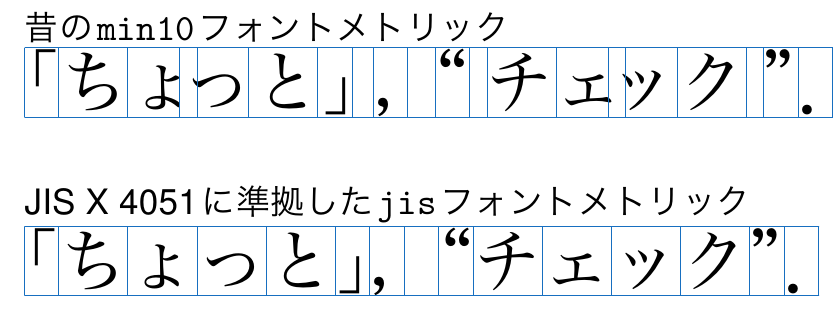
\includegraphics[width=.4\linewidth]{./image2012-gum/Okumura2011.png}
  \caption{日本語組版の例。上が{\pLaTeX}を用いた場合。下が奥村さんの新ドキュメントクラスを用いた場合(奥村, 2011)。}
  \label{fig:jisx0451}
  \vspace{-1em}
\end{figure}
句読点や括弧の処理が細かく調整されている様子が見てとれます。

最後に Unicode 対応について。
先ずお断りとして、{\TeX}における多言語処理についてはここでは割愛します\footnote{
  興味のある方は以下の URL を参照して下さい\\
  「pTeXと多言語処理」{\tt{\url{http://oku.edu.mie-u.ac.jp/~okumura/texwiki/?pTeX\%E3\%81\%A8\%E5\%A4\%9A\%E8\%A8\%80\%E8\%AA\%9E\%E5\%87\%A6\%E7\%90\%86}}}
}。
%
「ファイルの文字コードとして UTF-8 を使いたい」つまり「多言語混在の UTF-8 のファイルを直接処理したい」という
場合にも、最新の{\pLaTeX}(正確には $\varepsilon-$拡張がなされた $\varepsilon-$\pTeX)であれば、
そのまま処理できます。つまり、次の安定版(Wheezy)では、UTF-8 で保存されたソースをそのまま \pLaTeX で処理できるようになる……はずです%
(残念ながら squeeze では処理できません)。

\subsubsection{世界情勢}

ここで一端日本語を離れて、
日本語以外の{\TeX}(とその拡張)および多言語処理がどの様に発展しているのか、について簡単に触れてみましょう。
%
Knuthさんの{\TeX}開発終了宣言の後でも、
最下層の処理系としての{\TeX}は進化を続けており、$\varepsilon-$\TeX、そして pdf\TeX へと進展しています。
現在では{\LaTeX}として{pdf\LaTeX}が使われるのが一般的です
% \footnote{%%
%   お手元の環境で{\tt{latex}}と打ってみて下さい。おそらくエンジンとして{\tt{pdftex}}が起動するでしょう。
% }
。
pdf{\TeX}はその名の通り DVI ファイルを経ずに直接 PDF ファイルを出力する{\TeX}エンジンです。
この結果として、今後は DVI ファイルは過去の遺物になっていくのかもしれません
\footnote{
  これは日本語処理としてはある意味ありがたい話です。
  DVIファイルにはフォントの「参照」しか表れないため、表示が環境によって異なり、DeVice Independent が実現されません。
  PDF の場合はどうか、といえば、そもそも欧文のPDFの場合にはフォントを埋め込むのが一般的であり、
  和文のみが参照名({\tt{Ryumin-Light, GothicBBB-Medium}})のみで実フォントは埋め込まない、という状況でした。
  しかしながら、
  JIS2004前後で同じコードポイントに別のグリフが割り当てられているため、
  フォントを埋め込んでいない PDF では表示が異なる、という問題が発生します。
  %
  今後は欧文和文区別なく、フォントを埋め込んだ PDF を出力する、というのが一般的になるでしょう。
}
。
また、$\varepsilon-$\TeX は元々の \TeX に対して多くの拡張がなされています。
現在既に多くの拡張機能が$\varepsilon-${\TeX}に依存しているため、
$\varepsilon-${\TeX}に対応していないエンジンは時代遅れになりかねません%
\footnote{%
  幸いな事に北川弘典さんを中心に$\varepsilon-$\pTeX(=\pTeX + $\varepsilon-$TeX)が公開されており、
  TeXLive 本体にも同梱されています。本原稿執筆時点では既に
  Debian unstable で日本語環境を導入すると \pLaTeX のエンジンとして $\varepsilon-$\pTeX が使われています。
}

多言語処理系としては、壮大な試みであった$\Omega$が頓挫(?)した後、
現在ではXeTeX(=$\varepsilon-$\TeX + Unicode + OpenType) を用いるのが一般的になってきました。
Unicode での入出力を処理し、システムのフォントを利用して直接 PDF を出力します。
%
また、pdf{\TeX}の後継としてLua{\TeX}(pdf\TeX + $\Omega$ + Lua + METAPOST + OpenType)の開発が進められています。
Lua による柔軟な拡張が可能となっており、今後の進展が楽しみではあります。

なお、現時点では Xe(La)TeX および LuaTeX を用いて、
JIS X 4051 で規定された日本語の組版を実現するためには別パッケージが必要だったり、
プリアンブルをそれなりに修正する必要があるので一筋縄ではいきません。
%
今後に備えて動向を確認しておくのも良いでしょう
\footnote{
  \noindent
  XeTeX に関しては「XeLaTeXで日本語する件について」{\tt{\url{http://zrbabbler.sp.land.to/xelatex.html}}} \\
  LuaTeX-ja に関しては「LuaTeX-ja プロジェクト」{\tt{\url{http://sourceforge.jp/projects/luatex-ja/wiki/FrontPage}}}
}。

\subsubsection{{\TeX}Live について}

最後に、{\TeX}Liveについて。
{\TeX}に関するソフトウェアを提供する「ディストリビューション」として、以前は te\TeX がリリースされていました。
しかしながら、2009年に te\TeX としてリリースを停止した後\footnote{%
   teTeX: no next release
   「{\tt{\url{http://article.gmane.org/gmane.comp.tex.tetex.beta/812}}}」
}、
{\TeX}Live が{\TeX}のディストリビューションとしてリリースされるようになりました。
%
{\TeX}Live のリリースマネージャは Norbert Preining さんで、
彼は Debian の {\TeX} 関連パッケージのメンテナでもあります。
{\TeX}Live では {\tt{tpm2deb}} や {\tt{tpm2rpm}} といったパッケージ変換スクリプトも提供されており、
現在では多くの Linux ディストリビュータが {\TeX}Live を元に各々のパッケージを作成しています。
%
日本語関連については、2010年以降に {\TeX}Live本体への \pTeX、j{\TeX} のマージが開始され、
本原稿執筆時点では、patch の著作権者にコンタクトの取れていない {\tt{xdvik-ja}} 以外は
ほぼマージが完了しています。

\subsection{Debianにおける(日本語){\TeX}環境}

さてここまでのお話を踏まえた上で、ようやく Debian の{\TeX}環境について触れていきます。
%
ちなみに、「Debianでの{\pLaTeX}の設定」みたいな話はぐぐると結構でてくるので、あまり触れません
\footnote{%
  発表時および発表後は Q\&A および設定のお手伝いは行ないます。
}。

\subsubsection{Squeeze における(日本語){\TeX}環境}

Squeeze にて配布されている {\TeX}Live のバージョンは 2009 です。
ですので \pTeX および j{\TeX} 関連は、
$\varepsilon-$\TeX 拡張前の{\bf{UTF-8}}
のファイルを処理できないバージョンです。
具体的には、{\tt{ptex-buildsupport}} パッケージで te{\TeX}のソースを提供し、
これに patch を当てることで \pTeX や j{\TeX} のパッケージが構築されています。
%
また、ベースとなっているte{\TeX}のバージョンも 2007 であり、
セキュリティフィックスはなされているものの、
大雑把に言えば{\bf{2007年から更新されていません}}\footnote{%
  Squeeze リリース前に xdvik-ja の 64bit 対応の必要があり、
  佐々木が patch を当ててパッケージを再構築したりしました。
}。

導入後にも、
DVI ファイルの表示や PostScript/PDF への変換のために
幾つかおまじないが必要だったりします。
%
例えば
\begin{enumerate}
\item dvipsk-ja 用の VF ファイルの準備のために、インストール後に以下を唱える。
  \begin{commandline}
    $ sudo jisftconfig add
  \end{commandline}
  % $
\item xdvik-ja での表示のために
  \begin{commandline}
    # 明朝系の表示に使用するフォント
    $ fc-match serif:lang=ja
    # ゴシック系の表示に使用するフォント
    $ fc-match sans-serif:lang=ja
  \end{commandline}
  \noindent を確認し
  % \footnote{%
  %   {\tt{ttf-tamil-fonts}} や
  %   {\tt{ttf-devanagari-fonts}} がインストールされている場合には、
  %   これらが返ってきてしまい、
  %   結果として DVI の表示にこれらのフォントが使われる。
  % }
  、
  必要に応じて、{\tt{$\tilde{}$/.fonts.conf}} に
  {\tt{serif, sans-serif}}のエントリを追記して
  \begin{commandline}
    $ sudo update-vfontmap
  \end{commandline}
  % $
\item フォントが埋め込まれていない
  PDF の表示のために、{\tt{Ryumin, Gothic-BBB}}のエントリを
  {\tt{$\tilde{}$/.fonts.conf}}に追記する。
\item フォントを埋め込んだ PDF を生成するためには、
  {\tt{/etc/texmf/texmf.d/75DviPS.cnf}} の {\tt{TTFONTS}}、
  もしくは{\tt{\%OSFONTDIR}} に埋め込みたいフォントのパスを追加した後に
  \begin{commandline}
    $ sudo update-texmf
  \end{commandline}
  % $
  を唱えて、さらに map ファイルを適当に用意しておく。
\end{enumerate}
\vspace{-.8em}
などです。

\subsubsection{Squeezeで{\tt{{\TeX}Live(>=2011)}}を使う!?}

Debianのパッケージではありませんが、amd64 もしくは i386 の場合には
Norbert さんを中心に提供されている「tlptexlive リポジトリ\footnote{
  tlptexlive リポジトリ「{\tt{\url{http://tutimura.ath.cx/ptexlive/?tlptexlive\%A5\%EA\%A5\%DD\%A5\%B8\%A5\%C8\%A5\%EA}}}」
}」から、
TeXLive 全体のコンパイル済みバイナリを取得して使用する、という方法もあります。
%
この場合には
\begin{enumerate}
\item 既存の Debian パッケージの依存関係解消のために {\tt{equivs}} でダミーパッケージを作成する
\item {\TeX}Live のパッケージマネージャである{\tt{tlmpgr}}でのバイナリ導入先を、
  管理しやすい所に追いておく。
\end{enumerate}
なんて工夫が必要でしょう。佐々木は Squeeze 環境で
は {\tt{stow}} で tlptexlive リポジトリでのインストール物を管理しています。

ちなみに tlptexlive の配布物は {\tt{{\TeX}Live (>= 2011)}} 相当ですので、
フォント周りの設定は後述の Wheezy の場合と同じです。

\subsubsection{Wheezy の現状}

既に{\TeX}Live 2011(2012/dev) が Sid に upload されています。しかしながら、
本原稿執筆時点ではまだ Wheezy には更新された{\TeX}関連のパッケージは落ち
てきていません。
発表時には Wheezy に落ちてきていることを期待しつつ、
変更点を簡単に述べてみます。

このバージョンの {\TeX}Live には既に\pTeX などがマージされているため、
Squeeze までで提供していた te\TeX ベースのパッケージ群{\tt{ptex-bin, ptex-base, ...}}は軒並 obsolete となります\footnote{%
  {\TeX}Live 本体にマージされていない{\tt{xdvik-ja}}のみが残ることになります。
}。
%
現状では \pTeX 関連は {\tt{texlive-binaries, texlive-lang-cjk}} を導入することで一括で install される予定です。
また、フォント関連の扱いも {\tt{updmap-setup-kanji}} というコマンドによって、一括で設定できるようになります。
%
たとえば
\begin{commandline}
  $ sudo updmap-setup-kanji nofont
\end{commandline}
%$
\noindent といった塩梅です(上記の設定は、フォントをまったく埋め込まない場合です)。
このコマンドにより、{\tt{xdvik-ja, dvips, dvipdfmx}} のフォントマップが一括して更新されます。
%
{\TeX}Live ではフォントマップファイルとして、
1)埋め込まない場合、 2)IPAex を使う場合、3)ヒラギノを使う場合、4)小塚フォントを使う場合
の 4 つを提供しており、Debian のパッケージでもこれらのマップファイルを提供しています。
Debian の main セクションのみで作業をする場合には 1) or 2) を使うことになるでしょう。
現時点では、
\begin{itemize}
\item Conflicts, Replace, Provides の設定が半端で
  Squeeze からの upgrade がうまくできない(パッケージがある)。
\item {\TeX}Live 本体でも配布されているフォントがあり、
  既存のパッケージと重複しているため、Depends を追加して適宜 symbolic link に
  置換する必要がある。
\end{itemize}
といった問題があって、今後の修正が大変ですが、
Wheezy のリリースまでにはちゃんと直る(直す?)でしょう。

\subsection{最後に}

駆け足でしたが、日本語{\TeX}の現状および
Debian での{\TeX}関連の現状をまとめてみました。
%
まだまだ修正すべき点もありますが、
今後は{\tt{updmap-setup-kanji}}によるフォント関連の一括管理が有効になるため、
おまじないのような、
ともすればバッドノウハウと扱われがちな煩雑な設定は不要になるでしょう。
%
Wheezy からは、UTF-8 へ対応した \pTeX が、
もっと言えばJIX X 4051の組版要件を満たしつつ多言語処理も可能となった
日本語{\TeX}環境が非常に簡単に手に入るようになる予定です\footnote{%
  本来であればここで参考文献を列記すべきですが、
  紙面の都合上脚注に記す無作法をお許し下さい。
}。



%------------------------------------------------------------------------------
\dancersection{Linux-PAMの設定について}{西山和広}
\label{linux-pam}
\subsection{Introduction}
\label{sec-1-1}
\subsubsection{PAM とは何か?}
\label{sec-1-1-1}
%------------------------------------------------------------------------------

Linux-PAM (Pluggable Authentication Modules for Linux) とは、アプリケーションがユーザーをどう認証するかをローカルシステムの管理者が設定できるようにするための共有ライブラリ一式です。

PAM のおかげで、アプリケーションをコンパイルしなおさなくても、認証方法を変更したり、権限の付与の仕方を変更したりできるようになっています。
\subsubsection{NSS とは何か?}
\label{sec-1-1-2}

PAM と関係の深いライブラリとして NSS (Name Service Switch) があります。
NSS はユーザー名とユーザー ID との変換をしたり、ホスト名と IP アドレスとの変換をしたりするときに使われます。
\subsubsection{PAM と NSS との違い}
\label{sec-1-1-3}

PAM は認証部分のみなので、基本的にはログインやログアウトのときとパスワード変更に関係します。 (厳密にはアプリケーション次第です。)

ログイン中に \verb~id~ コマンドで表示されるユーザーIDとユーザー名の対応 \footnote{グループIDとグループ名も同様です。 } や \verb~ls -l~ でファイルシステムに記録されているユーザーIDからユーザー名への変換 \footnote{ファイルシステムには所有者はユーザーIDで記録されています。そのため、たとえばユーザーを削除して存在しないユーザーのファイルがある場合には、ユーザー名への変換が出来ないので数字で表示されます。 } などは \verb~/etc/nsswitch.conf~ で設定する NSS の機能になります。
\subsubsection{PAM の設定}
\label{sec-1-1-4}

PAM は設定ファイルに実行したいモジュールを並べておいて、それを順番に実行していくようなものだと思えば良いでしょう。

たとえば、
\begin{itemize}
\item \verb~/etc/passwd~ などのローカルファイルでの認証
\begin{itemize}
\item 成功すれば認証成功をアプリケーションに返す
\item 失敗すれば次へ
\end{itemize}
\item LDAP での認証
\begin{itemize}
\item 成功すれば認証成功をアプリケーションに返す
\item 失敗すれば次へ
\end{itemize}
\item 次がないので認証失敗をアプリケーションに返す
\end{itemize}
という動作をします。
\subsection{ファイル配置}
\label{sec-1-2}
\subsubsection{設定ファイル}
\label{sec-1-2-1}

\verb~/etc/pam.d/~ の下にアプリケーションごとの設定ファイルがあります。
以下はその例です。


\begin{commandline}
$ ls /etc/pam.d
atd       chsh            common-password                cron      other   su
chfn      common-account  common-session                 login     passwd  sudo
chpasswd  common-auth     common-session-noninteractive  newusers  sshd
\end{commandline}
%$

\begin{itemize}
\item どの設定ファイルがどのアプリケーションのものなのかはファイル名から推測できます
\item ない場合は \verb~other~ が使われます
\item それぞれの中から \verb~@include~ で \verb~common-*~ で共通の設定を使うようになっています
\end{itemize}

\verb~/etc/pam.d/~ がない場合は \verb~/etc/pam.conf~ が使われると \verb~/etc/pam.conf~ の中のコメントに書いてありますが、この記述は歴史的なもので最近の Linux では使われていません。
\subsubsection{モジュール}
\label{sec-1-2-2}

以下は PAM モジュールの例です。


\begin{commandline}
$ ls /lib/x86_64-linux-gnu/security
pam_access.so     pam_keyinit.so    pam_nologin.so     pam_tally.so
pam_debug.so      pam_lastlog.so    pam_permit.so      pam_tally2.so
pam_deny.so       pam_ldap.so       pam_pwhistory.so   pam_time.so
pam_echo.so       pam_limits.so     pam_rhosts.so      pam_timestamp.so
pam_env.so        pam_listfile.so   pam_rootok.so      pam_umask.so
pam_exec.so       pam_localuser.so  pam_securetty.so   pam_unix.so
pam_faildelay.so  pam_loginuid.so   pam_selinux.so     pam_userdb.so
pam_filter.so     pam_mail.so       pam_sepermit.so    pam_warn.so
pam_ftp.so        pam_mkhomedir.so  pam_shells.so      pam_wheel.so
pam_group.so      pam_motd.so       pam_stress.so      pam_xauth.so
pam_issue.so      pam_namespace.so  pam_succeed_if.so
\end{commandline}
%$

\begin{itemize}
\item 設定ファイルに書かれる \verb~pam_unix.so~ などは \verb~dlopen(3)~ で動的に読み込まれます
\item そのため PAM の認証を使っているプログラムを入れた chroot 環境を作るときには気をつける必要があります
\item \verb~squeeze~ までは \verb~/lib/security/~ や \verb~/lib64/security/~ にあります
\item \verb~multiarch~ 対応で最近は \verb~/lib/x86_64-linux-gnu/security/~ などの \verb~/lib/<triplet>/security/~ にあります。
  上記の例は wheezy (testing) なので \verb~/lib/security/~ ではなく
  \verb~/lib/x86_64-linux-gnu/security/~ になっています
\end{itemize}
\subsection{設定ファイルの書式}
\label{sec-1-3}

設定ファイルの例を載せておきます。(一部省略)

\begin{commandline}
$ egrep '^[^#]' /etc/pam.d/cron
@include common-auth
session       required   pam_env.so
session       required   pam_env.so envfile=/etc/default/locale
@include common-account
@include common-session-noninteractive
session    required   pam_limits.so
\end{commandline}
%$

\begin{itemize}
\item 設定ファイルには以下の項目を指定します。詳細は後述します
\begin{description}
\item[\verb~service~] アプリケーションに対応する名前
\item[\verb~type~] PAM の分類
\item[\verb~control~] 動作指定
\item[\verb~modules-path~] PAM モジュールへのパス
\item[\verb~module-arguments~] PAM モジュールの引数
\end{description}
\item \verb~#~ から行末まではコメントになります
\item \verb~\~ が改行 (\verb~<LF>~) の直前にあると継続行になります
\item \verb~/etc/pam.conf~ では「 \verb~service type control module-path module-arguments~ 」という書式で設定します。( \verb~service~, \verb~type~, \verb~control~ の大文字小文字は無視されます。)
\item \verb~/etc/pam.d/~ では \verb~service~ がファイル名 (必ず小文字) になります
\item 残りの「 \verb~type control module-path module-arguments~ 」がファイルの内容になります
\end{itemize}
\subsubsection{service}
\label{sec-1-3-1}

\begin{itemize}
\item \verb~service~ は具体的には \verb~login~ や \verb~su~ になります
\item \verb~other~ という \verb~service~ 名はデフォルト設定用として予約されています
\item Debian では \verb~common-~ で始まる名前のファイルが共通設定用のファイルになっていて、他の設定ファイルから \verb~@include~ で読み込まれています
\end{itemize}
\subsubsection{type}
\label{sec-1-3-2}

\begin{description}
\item[account] 認証以外のアカウント管理に使われます。たとえば昼間だけログインできるようにしたり、 \verb~nologin~ ファイルがあるときは一般ユーザーにログインさせないようにしたりできます
\item[auth] アプリケーションにパスワード入力を要求するなどの方法でユーザー認証をします。グループ権限の付与などの機能もあります
\item[password] パスワード変更などの認証トークン変更機能を提供します
\item[session] サービス利用の前後に何かをするモジュールタイプです。ログを取ったり、ディレクトリをマウントしたり、 \verb~/etc/motd~ を表示したり、環境変数を設定したりできます
\item[\verb~@include~] Debian ではここに \verb~@include~ を指定することで別のファイルを読み込めるようになっています
\end{description}
\subsubsection{control}
\label{sec-1-3-3}

PAM モジュールを実行してその結果、どうするのかの設定です。
詳細については後述します。
\subsubsection{module-path}
\label{sec-1-3-4}

PAM モジュールのファイルへのパスを絶対パスかデフォルトのモジュールの置き場所である \verb~/lib/security/~ などからの相対パスで指定します。
\subsubsection{module-arguments}
\label{sec-1-3-5}

スペース区切りでモジュールへの引数を指定します。
スペースを含む引数を指定する場合は以下の例のように \verb~[]~ でくくります。


\begin{commandline}
squid auth required pam_mysql.so user=passwd_query passwd=mada \
      db=eminence [query=select user_name from internet_service \
      where user_name='%u' and password=PASSWORD('%p') and \
      service='web_proxy']
\end{commandline}

\verb~]~ を含めたい場合は \verb~\]~ と指定します。
つまり以下のようになります。


\begin{commandline}
[..[..\]..]    -->   ..[..]..
\end{commandline}
\subsection{control の設定について}
\label{sec-1-4}
\subsubsection{PAM の内部状態}
\label{sec-1-4-1}

PAM はモジュールを実行していくときに内部的に
\begin{itemize}
\item 初期状態
\item 成功状態
\item 失敗状態
\end{itemize}
の3つの状態があり、最終的に成功状態なら成功をアプリケーションに返し、そうでなければ失敗をアプリケーションに返します。
(初期状態のままのときも失敗を返します。)
\subsubsection{control の省略形式}
\label{sec-1-4-2}

control の指定には、省略した形式として以下のものがあります。

\begin{description}
\item[required] 成功しても失敗しても続きを実行してから結果を返します。失敗状態以外で成功した場合は成功状態にします。失敗した場合は失敗状態にします
\item[requisite] 失敗した場合は失敗状態にして、すぐにアプリケーションに失敗を返します。失敗状態以外で成功した場合は成功状態にします
\item[sufficient] 失敗状態以外で成功した場合は、すぐにアプリケーションに成功を返します。失敗は無視して続きを実行します
\item[optional] 成功か失敗かは気にせず実行したいモジュールに使います。成功か失敗かは他のモジュールがないときだけ影響します
\item[include, substack] 省略形式ではありませんが、このような指定も出来ます。しかし Debian では上述の \verb~@include~ が使われていて、これらは普通は使われていないのと、内部状態の説明が複雑になるため省略します
\end{description}
\subsubsection{control の省略しない形式}
\label{sec-1-4-3}

もっと複雑な形式として以下のものがあります。


\begin{commandline}
[value1=action1 value2=action2 ...]
\end{commandline}
\subsubsection{control の value}
\label{sec-1-4-4}

\verb~valueN~ は PAM モジュールからの返値で \verb~actionN~ はその返値のときにどうするかという設定です。
\verb~valueN~ には、

{\scriptsize
\begin{tabular}{cc}
  \begin{minipage}[b]{0.3\textwidth}
    \begin{itemize}
    \item \verb~success~
    \item \verb~open_err~
    \item \verb~symbol_err~
    \item \verb~service_err~
    \item \verb~system_err~
    \item \verb~buf_err~
    \item \verb~perm_denied~
    \item \verb~auth_err~
    \item \verb~cred_insufficient~
    \item \verb~authinfo_unavail~
    \item \verb~user_unknown~
    \end{itemize}
  \end{minipage}
  \begin{minipage}[b]{0.3\textwidth}
    \begin{itemize}
    \item \verb~maxtries~
    \item \verb~new_authtok_reqd~
    \item \verb~acct_expired~
    \item \verb~session_err~
    \item \verb~cred_unavail~
    \item \verb~cred_expired~
    \item \verb~cred_err~
    \item \verb~no_module_data~
    \item \verb~conv_err~
    \item \verb~authtok_err~
    \item \verb~authtok_recover_err~
    \end{itemize}
  \end{minipage}
  \begin{minipage}[b]{0.3\textwidth}
    \begin{itemize}
    \item \verb~authtok_lock_busy~
    \item \verb~authtok_disable_aging~
    \item \verb~try_again~
    \item \verb~ignore~
    \item \verb~abort~
    \item \verb~authtok_expired~
    \item \verb~module_unknown~
    \item \verb~bad_item~
    \item \verb~conv_again~
    \item \verb~incomplete~
    \item \verb~default~
    \end{itemize}
  \end{minipage}
\end{tabular}
}

が指定できます。
\verb~default~ は名前からわかる通り明示的に \verb~valueN~ に指定されなかったときのデフォルト指定です。

\verb~valueN~ に指定できる値の完全なリストは \verb~libpam0g-dev~ パッケージをインストールして
\begin{itemize}
\item \verb~/usr/include/security/_pam_types.h~
\end{itemize}
を参照してください。
\subsubsection{control の action}
\label{sec-1-4-5}

\verb~actionN~ に指定できるものは以下の通りです。

\begin{description}
\item[ignore] 無視します。モジュールの返値はアプリケーションに返す値には影響しません
\item[bad] 失敗状態にします
\item[die] 失敗します。失敗状態にして、すぐにアプリケーションに失敗を返します
\item[ok] 失敗状態以外なら成功状態にします。すでに失敗状態のときは失敗状態のままです
\item[done] 失敗状態以外なら成功状態にして、すぐにアプリケーションに成功を返します。すでに失敗状態のときは失敗状態のままです
\item[N (1以上の整数)] 次の N 個のモジュールを実行せずに飛ばします
\item[reset] 内部状態を初期状態に戻します
\end{description}
\subsubsection{省略形の展開}
\label{sec-1-4-6}

省略形は \verb~[...]~ の書式で書くと以下のようになります。

\begin{description}
\item[required] \verb~[success=ok new_authtok_reqd=ok ignore=ignore default=bad]~
\item[requisite] \verb~[success=ok new_authtok_reqd=ok ignore=ignore default=die]~
\item[sufficient] \verb~[success=done new_authtok_reqd=done default=ignore]~
\item[optional] \verb~[success=ok new_authtok_reqd=ok default=ignore]~
\end{description}
\subsection{PAM 設定フレームワーク}
\label{sec-1-5}

Red Hat 系 Linux には以前から PAM や NSS の自動設定用のコマンドとして \verb~authconfig~ があります。
しかし、昔の Debian にはそういうフレームワークはありませんでした。

Ubuntu では、そのようなフレームワークとして \verb~auth-client-config~ が使われるようになりました。
その後 \verb~pam-auth-update~ が使われるように変わりました。
そして Debian にも \verb~pam-auth-update~ が入って今は Debian でも Ubuntu でも \verb~pam-auth-update~ が標準の PAM の設定用フレームワークとして使われています。\footnote{Debian にはありませんが、 Ubuntu には \verb~auth-client-config~ パッケージはまだ存在しています。 \verb~pam-auth-update~ は PAM の設定のみなので、もしかすると NSS の設定には使われているのかもしれません。(使っていないので詳細は不明です。) }
\subsubsection{pam-auth-update}
\label{sec-1-5-1}

\verb~pam-auth-update~ コマンドは \verb~libpam-runtime~ パッケージに入っています。
PAM モジュールパッケージで \verb~/usr/share/pam-configs~ の中にプロファイルがインストールされます。
\verb~pam-auth-update~ コマンドは、そのプロファイルを元に \verb~/etc/pam.d/common-*~ ファイルを更新します。
\subsection{設定ファイルの例}
\label{sec-1-6}

\begin{itemize}
\item \verb~pam-auth-update~ で生成された設定ファイルの一部と sshd の設定を例として説明をします。
\end{itemize}
\subsubsection{/etc/pam.d/common-auth}
\label{sec-1-6-1}

common-auth は認証の共通処理の設定ファイルです。
\begin{enumerate}
\item まず最初に ``Primary'' block のモジュールを \verb~pam_unix.so~, \verb~pam_ldap.so~ と順番に試して、どこかで成功したら \verb~pam_permit.so~ まで飛ばして成功状態にします
\item すべて失敗した場合は fallback の \verb~pam_deny.so~ の行で必ず失敗して、そのままアプリケーションに認証失敗を返します
\item 途中で成功して \verb~pam_permit.so~ の行に飛んできた場合は、そのまま続きの行を実行していきます
\item \verb~@include~ 元のファイルで続きの処理を用意していることもあるので \verb~sufficient~ で成功をすぐに返してしまうことは避けて \verb~success=N~ で飛ばして \verb~pam_permit.so~ で成功状態にするという手間をかけているようです
\item \verb~pam_ldap.so~ の \verb~use_first_pass~ は \verb~pam_unix.so~ の認証のときに入力されたパスワードを使って \verb~pam_ldap.so~ の認証も試すという意味です。 \verb~use_first_pass~ がないと \verb~pam_unix.so~ でパスワード入力が要求されて、さらに \verb~pam_ldap.so~ でもパスワード入力を要求されるということになります。(プロファイルで Auth-Initial と Auth にわかれているのはそういう設定を使いわけられるようにするためのようです。)
\end{enumerate}

\begin{commandline}
# here are the per-package modules (the "Primary" block)
auth    [success=2 default=ignore]      pam_unix.so nullok_secure
auth    [success=1 default=ignore]      pam_ldap.so minimum_uid=1000 use_first_pass
# here's the fallback if no module succeeds
auth    requisite                       pam_deny.so
# prime the stack with a positive return value if there isn't one already;
# this avoids us returning an error just because nothing sets a success code
# since the modules above will each just jump around
auth    required                        pam_permit.so
# and here are more per-package modules (the "Additional" block)
auth    optional                        pam_cap.so
# end of pam-auth-update config
\end{commandline}
\subsubsection{/etc/pam.d/common-session}
\label{sec-1-6-2}

\begin{itemize}
\item この例の common-session では ``Primary'' block にモジュールがないために \verb~pam_permit.so~ でいきなり \verb~pam_deny.so~ を飛びこえるようになっています
\item その後 \verb~pam_unix.so~ と \verb~pam_ldap.so~ でも何か追加の処理をして \verb~pam_tmpdir.so~ で環境変数 TMPDIR などを設定しています
\end{itemize}

\begin{commandline}
# here are the per-package modules (the "Primary" block)
session [default=1]                     pam_permit.so
# here's the fallback if no module succeeds
session requisite                       pam_deny.so
# prime the stack with a positive return value if there isn't one already;
# this avoids us returning an error just because nothing sets a success code
# since the modules above will each just jump around
session required                        pam_permit.so
# and here are more per-package modules (the "Additional" block)
session required        pam_unix.so
session [success=ok default=ignore]     pam_ldap.so minimum_uid=1000
session optional pam_tmpdir.so
# end of pam-auth-update config
\end{commandline}
\subsubsection{/etc/pam.d/sshd}
\label{sec-1-6-3}

\begin{enumerate}
\item まず \verb~pam_env.so~ で環境変数を設定しています
\item \verb~#~ で始まる行だけでなく、行の途中の \verb~#~ 以降もコメントです
\item 2個目の \verb~pam_env.so~ で \verb~/etc/default/locale~ を読み込んでいます \footnote{余談ですが、昔の Debian では \verb~/etc/default/locale~ は存在しなくて、アップグレードでも自動で作成はされず、ログをみるとエラーが出ていたということがあり、そのときは自分で \verb~/etc/default/locale~ を作成しました。今は \verb~update-locale~ というコマンドで更新するとチェックもしてくれて良い感じになるようです。 }
\item \verb~pam_nologin.so~ では \verb~nologin~ ファイルがあるときにログインを認可しないようにしています
\item session では \verb~pam_motd.so~ で \verb~/etc/motd~ の表示をしています。最近の Debian や Ubuntu の \verb~pam_motd.so~ では \verb~/etc/update-motd.d~ があれば表示前に内容が更新されるようになっています。 Ubuntu のサーバーに ssh でログインしたときにいろいろな情報がでるのはそのためです。 Ubuntu の場合は update-notifier-common を入れておくとパッケージの更新や再起動が必要かどうかが ssh などでのログイン時に出るようになるのでおすすめです。 Debian では \verb~/etc/update-motd.d~ のファイルが入らない ( \href{http://bugs.debian.org/580286}{http://bugs.debian.org/580286} ) ため、自動では出ません
\item 他にはメールボックスの状態を表示したり、リソース制限を反映したりしているようです
\end{enumerate}

\begin{commandline}
# PAM configuration for the Secure Shell service

# Read environment variables from /etc/environment and
# /etc/security/pam_env.conf.
auth       required     pam_env.so # [1]
# In Debian 4.0 (etch), locale-related environment variables were moved to
# /etc/default/locale, so read that as well.
auth       required     pam_env.so envfile=/etc/default/locale

# Standard Un*x authentication.
@include common-auth

# Disallow non-root logins when /etc/nologin exists.
account    required     pam_nologin.so

# Uncomment and edit /etc/security/access.conf if you need to set complex
# access limits that are hard to express in sshd_config.
# account  required     pam_access.so

# Standard Un*x authorization.
@include common-account

# Standard Un*x session setup and teardown.
@include common-session

# Print the message of the day upon successful login.
session    optional     pam_motd.so # [1]

# Print the status of the user's mailbox upon successful login.
session    optional     pam_mail.so standard noenv # [1]

# Set up user limits from /etc/security/limits.conf.
session    required     pam_limits.so

# Set up SELinux capabilities (need modified pam)
# session  required     pam_selinux.so multiple

# Standard Un*x password updating.
@include common-password
\end{commandline}
\subsection{設定変更時の注意事項}
\label{sec-1-7}

設定を変更するときは root 権限のシェルを開いたままにしておくことをお勧めします。
もし設定を間違えてしまうと sudo も su もコンソールからの root でのログインも出来なくなって困ることになります。

ただし \verb~pam-auth-update~ を使ってパッケージでインストールされた設定の有効無効を切り替えるだけの場合は問題が起きる可能性は低いので、そこまでしなくても普通は大丈夫だと思います。
\subsection{参考文献}
\label{sec-1-8}

\begin{itemize}
\item \href{http://linux-pam.org/Linux-PAM-html/Linux-PAM_SAG.html}{http://linux-pam.org/Linux-PAM-html/Linux-PAM\_SAG.html} The Linux-PAM System Administrators' Guide Version 1.1.2, 31. August 2010
\item \href{http://archive.linux.or.jp/JF/JFdocs/User-Authentication-HOWTO/}{http://archive.linux.or.jp/JF/JFdocs/User-Authentication-HOWTO/} User Authentication HOWTO 2000/05/02
\item \href{https://wiki.ubuntu.com/PAMConfigFrameworkSpec}{https://wiki.ubuntu.com/PAMConfigFrameworkSpec} PAMConfigFrameworkSpec - Ubuntu Wiki
\item \href{https://wiki.ubuntu.com/AuthClientConfig}{https://wiki.ubuntu.com/AuthClientConfig} AuthClientConfig - Ubuntu Wiki
\end{itemize}


%------------------------------------------------------------------------------
\dancersection{数学ソフトウェア使ってますか?}{濱田龍義}
\label{sec:MathLibre}
%------------------------------------------------------------------------------

\vspace{2em}
% add upper space for logo

Debian パッケージには「数学」というセクションが存在し、多数の数学ソフト
ウェアが提供されています。 一方で、パッケージには未収録ですが、
数学の研究、教育の現場で使われているフリーソフトウェアが
世界中で開発されています。
2003年頃から、このような数学ソフトウェアをライブCDであるKNOPPIX に収録して紹
介してきたプロジェクトが KNOPPIX/Math です。
KNOPPIX は Debian をベースに、ドイツの Klaus Knopper によって開発が進
められている Live Linux です。当初は CD 起動のみに対応していましたが、
DVD や USB メモリーディスクにも対応し、現在も開発が進められています。
KNOPPIX/Math では、2006年から LiveDVD を採用しました。
また、2012年からは KNOPPIX 以外のシステムの利用も考慮し、
MathLibreとプロジェクト名を変更しています。
本講演では MathLibre に収録している様々な数学ソフトウェアから、
いくつかを紹介します。

\subsection{数学ソフトウェアの歴史}
我々は、数学を取り扱うもの、また、数学に関連するもの、そういったものすべ
てを数学ソフトウェアと呼んでいます。
%例えば、前の佐々木先生の講演では\TeX{}(\TeX{}Live) が取り上げられました。
Donald E. Knuth によって生み出された組版システム \TeX{}は、
数学を生業とするものにとっては、欠かせない道具であり、
これもまた、数学ソフトウェアの一種です。
一般的に、数式処理ソフトウェア、数値計算ライブラリ、可視化ツールなども
数学ソフトウェアと考えて良いでしょう。

その中で、数式処理ソフトウェアと呼ばれるソフトウェアについて紹介します。
Debian のオフィシャルパッケージの中で、比較的使いやすい物としては、
Maxima が有名です。Maxima の原型は MACSYMA と呼ばれるシステムで、
1960年代に MIT の人工知能研究グループによって開発されました。
1980年代には MACSYMA は商用ソフトウェアとしても流通していましたが、
現在の Maxima は、William Schelter によって GNU Common Lisp 上に実装され
たものを原型に2001年にGPL化され、Maxima と名称を改めて、
フリーソフトウェアとして公開されたものです。
Maximaは、方程式の求解、多項式の因数分解、初等函数の微積分、
行列計算、グラフの描画等に対応しています。中でも積分アルゴリズムの実装につ
いて評価が高いようです。

Debian 上で Maxima を起動するための命令は {\tt maxima} です。
\begin{commandline}
knoppix@Microknoppix:~$ maxima

Maxima 5.26.0 http://maxima.sourceforge.net
using Lisp GNU Common Lisp (GCL) GCL 2.6.7 (a.k.a。GCL)
Distributed under the GNU Public License。See the file COPYING.
Dedicated to the memory of William Schelter.
The function bug_report() provides bug reporting information.
(%i1) integrate(1/(x^3+1),x);
                                         2 x - 1
                       2            atan(-------)
                  log(x  - x + 1)        sqrt(3)    log(x + 1)
(%o1)           - --------------- + ------------- + ----------
                         6             sqrt(3)          3
(%i2)
\end{commandline}
%$

\subsubsection{Maximaのユーザインターフェース}
コマンドラインからの利用が一番速く手軽ですが、
一般的なグラフィカルユーザインターフェースとしては、
XMaxima ({\tt xmaxima}) や WxMaxima ({\tt wxmaxima}) が存在します。
XMaxima は Tcl/Tk, WxMaxima は WxWidget によって
実装されています。また、Emacs 用に便利なインターフェースとしては
imaxima ({\tt maxima-emacs}) が存在します。
Emacs 上で {\tt M-x imaxima} で起動すると、
数式の計算結果を \TeX{} スタイルに整形された形で出力されます。
また、少し変わったインターフェースとしては GNU TeXmacs ({\tt texmacs})と呼ばれる
科学技術計算用ワードプロセッサが存在します。
こちらも計算結果の出力を整形された形で表示することができます。

\begin{center}
\begin{figure}[ht]
\begin{minipage}[c]{8cm}
  \includegraphics[width=1\hsize]{image2012-gum/imaxima.eps}
  \caption{imaxima on Emacs}
  \label{fig:imaxima}
\end{minipage}
\begin{minipage}[c]{8cm}
  \includegraphics[width=1\hsize]{image2012-gum/texmacs.eps}
  \caption{GNU TeXmacs}
  \label{fig:texmacs}
\end{minipage}
\end{figure}
\end{center}

Maxima と同じく、長い歴史を持つ数式処理システムとしては、Reduce もよく知られ
た存在です。
Reduce もまた、1960年代に開発が始められたシステムですが、こちらは
理論物理学からの要請により開発されました。
Reduce も MACSYMA と同様に1980年代に商品化され、日本では差分方程式論、
および可積分系等の分野で多くのユーザを獲得しています。
その後、2009年に Reduce は Tony Hearn によって BSD ライセンスで公開され、
現在に至ります。
まだ、Debian オフィシャルパッケージには含まれていませんが、
getdeb ({\tt \url{http://www.getdeb.net/}})から、パッケージが入手可能です。
Reduce もまた、微分方程式の求解、積分、行列計算、グラフの描画等に対応し
ています。

Maxima も Reduce も、たいへん歴史の古いソフトウェアであり、
現在も、多くのユーザを獲得し、開発グループが日夜、
更新を続けているソフトウェアです。
その他にも、数論の PARI/GP、群論の GAP、統計計算の R、可換環論の Singular、Macaulay2等が研究ツールとして有名です。PARI/GP、GAP、R はオフィシャルパッケージに
なっていますが、Singular、Macaulay2 については、上流開発者によるパッケー
ジは提供されていますが、オフィシャルには収録されていません。

一方、日本国内における数式処理システムの開発については、
1970年代に日本電信電話会社で AL が、1980年代に
理研で GAL が開発されました。また、1980年代末に、
富士通研究所で開発された Risa/Asir は、現在、拠点を
神戸大学に移して、研究、開発が進められています。特にグレブナー基底等、
多項式の計算に特化して、高速計算が可能であり、
MathLibre プロジェクトの中心的な存在として収録されています。
ただ、Risa/Asir は富士通研究所時代のライセンスを引き継いでおり、
オープンソースソフトウェアライセンスとは
異なるライセンスで配布されています。

\subsection{最近のシステム}
ここで、最近の動きに注目して、いくつかの数学ソフトウェアを紹介します。
\subsubsection{Sage}
Sage は2005年に William Stein によって開始されたオープンソースプロジェクトです。
彼が Sage の開発を始めた背景については
``Mathematical Software and Me: A Very Personal Recollection'' \cite{stein}に
詳しく述べられています。
現在、Sage は数学者を始めとする大勢の専門家によって開発が進められていま
す。2007年にはフリーソフトウェアの賞である
Les Troph\'{e}es du Libre の科学技術部門において金賞を受賞しています。
Sage Days と呼ばれるイベントを世界各地で開催しており、開発者と
利用者からなる巨大なコミュニティが存在します。
先日、九州大学において日本で初の Sage Days が開催され、多くの
参加者を得ました。

Sage は「車輪の再発明」はしないということを掲げており、
既に実績のある Maxima や Singular、PARI/GP、GAP、R といった
数学ソフトウェアを組み合わせることで、使いやすい環境の構築を
目指しています。それぞれの数学ソフトウェアをつなぎ合わせているのは
オブジェクト指向プログラミング言語 Python です。
Python 自身もオープンソースソフトウェアですが、世界中で熱狂的な利用者、開発者を
獲得しています。その使いやすさと、多機能性から
さまざまなプロジェクトが Python で開発されています。
それまでは、数学ソフトウェアを使いこなすためには、
そのソフトウェアごとに異なるプログラミング機能を活用しなければいけなかったのですが、
Sage は Python という一般的なプログラミング言語を
用いることで、統一的なインターフェースを提供しています。また、
Python のオブジェクト指向言語としての機能を活用できる点も
魅力となっているようです。
Sage Notebook と呼ばれるユーザーインターフェースを提供しており、
Mozilla Firefox 等の
Webブラウザ上で数式処理やグラフ描画といった機能を利用することができます。

Sageについての入門書としては、Ted Kosan による ``Sage for Newbies''
\cite{newbie} が良く知られています。これは横田博史氏によって「はじめての
Sage」\cite{ponpoko}として翻訳され、MathLibre にも収録されています。
最近、韓国では大学初年級の微分積分と線形代数について Sage を用いて解説した書籍が
出版されました。

Sage は、あまりに巨大なシステムであり、更新も頻繁であるため、
現在は、Debian パッケージとして配布されていません。Linux 用には
バイナリー版が配られています。多少の時間はかかりますが、CPUごとに最適化する
ため、ソースからコンパイルすることをお勧めします。
Windows 版については、以前は仮想マシンの Ubuntu 上で起動したサーバに
Windows 上のブラウザから接続する形式だったのですが、現在は、
Fedora Core 上で起動したサーバに Fedora Core 上の Chrome を接続させる
形になったようです。

\begin{figure}[ht]
\begin{minipage}[c]{0.45\hsize}
\includegraphics[height=0.8\hsize]{image2012-gum/sage.eps}
\caption{Sage によるグラフ描画}
\label{fig:sage}
\end{minipage}
\begin{minipage}[c]{0.48\hsize}
\includegraphics[height=0.72\hsize]{image2012-gum/taylor.eps}
\caption{GeoGebra によるテイラー多項式}
\label{fig:geogebra}
\end{minipage}
\end{figure}


\subsubsection{GeoGebra}
GeoGebra はオーストリアのヨハネスケプラー大学の Markus Hohenwarter によって
始められた数学ソフトウェアプロジェクトです。
彼はザルツブルク大学の学生時代に
テキサス・インスツルメンツ社の電卓 TI-92 Plus に触れる機会を持ちました。
彼は電卓に収録されていた動的幾何ソフト Cabri Geometry
と数式処理システム Derive に刺激を受けて開発を志したということです\cite{markus}。
2001年2月に最初のプロトタイプを開発し、
2002年3月には GeoGebra の開発でコンピュータサイエンスと数学教育に関する
修士号を取得しています.
この間、GeoGebra は、各国で数多くの賞を受賞しています。
2004年から2006年にかけては数学教育に関する PhD プロジェクトとして開発が
進められ、Austiran Academy of Sciences から支援を受けて、着実にその存在
を世界中に知らしめました。
GeoGebra もまた、オープンソースソフトウェアとして公開されています。
Java の実行環境を必要としますが、Windows、MacOS X、Linux 等、計算機環境を問わ
ずに利用可能です。Debian では stable に 3.2 系が testing に 4.0 系が
収録されています。

GeoGebra は起動すると ``Dynamic Mathematics for Everyone'' というメッセージ
を表示します。日本語に訳すと「動的数学ソフトウェア」でしょうか。
これは GeoGebra が Cabri や Cinderella と言った
動的幾何学ソフトウェア(Dynamic Geometry Software)
と呼ばれるソフトウェアの影響を受けていること、
また、主要なユーザインターフェースが動的幾何学ソフトウェアとしての機能を備えていることから類推されます。
GeoGebra という名称は幾何学(Geometry)+ 代数学(Algebra)という意の造語です.開発初期の段階では GeoGebra は動的幾何学ソフトウェアとしての機能しか持ちませんでした。しかし、現在では関数入力によるグラフ描画、数式処理、スライダー、表計算機能等を備えており、幾何学ソフトウェアという枠組みだけでは語り尽くせない存在です。

メニューやヘルプ、マニュアル等の翻訳についても世界中のボランティアスタッ
フによって活発に行われており、最新の GeoGebra 4.0 では約50ヵ国語に対応しました。
日本語化については、北海道教育大学の和地輝仁氏が中心となって進めており,
国内のユーザーを増やすきっかけとなっています。
%韓国語版については、Gyeonggi-Buk Science High School の Choi Kyeong-Sik によって翻訳が進められており、Naver という韓国最大手のインターネット検索ポータルサイトに GeoGebra のコミュニティを形成し普及に努めているようです。

GeoGebra は動的幾何学ソフトウェアとしての機能と
グラフ描画ソフトの機能が連携することで使い易いインターフェースを提供しています.
また、Maxima や Reduce と連携して数式処理機能を備えているため、
微分や積分、因数分解等の基本的な演算にも対応しています。
図 \ref{fig:geogebra} のようにグラフ上の点を動的に動かしてテイラー多項式によって描かれるグラフを観察することもできます。

表計算ビューを備えたことで、統計方面についても
機能が強化されており、教材作成に威力を発揮するものと思われます。
すべての機能を述べることはできませんが、
ヘルプやさまざまなサンプル、ムービー等も豊富で、
初めての方でも使いやすい数学ソフトウェアだと思います。
どちらかと言えば、研究よりも数学教育に焦点をあてたソフトウェアですが、
その使いやすいインターフェースから構成される可視化機能は、
プレゼンテーションなどでも威力を発揮するでしょう。
次期バージョンの4.2では本格的な数式処理シェルを備え、
5.0では3Dに対応する予定です。
潜在的な能力も含めて今後の展開が楽しみな数学ソフトウェアです。

2012年7月4日--6日にはRIMS共同研究「数式処理研究の新たな発展」が
計画されていますが、7月5日に GeoGebra Institute から
Zsolt Lavizca, Bal\'azs Koren の2人が GeoGebra の最新事情についての講演
が行われます。

\subsection{まとめ}
ここに紹介したソフトウェアは、MathLibre に収録している100以上の
数学ソフトウェアのごく一部です。本稿が、数学ソフトウェアに
興味を持っていただくきっかけになれば幸いです。

\begin{thebibliography}{99}
%\bibitem{stein1}
%David Joyner and William Stein,
%\emph{Open source mathematical software},
%Notices of the AMS、\textbf{54} (3) (2007),
%http://www.ams.org/notices/200710/tx071001279p.pdf

\bibitem{stein}
William Stein,
``\emph{Mathematical software and me:A very personal recollection}'',
\url{http://wstein.org/}

\bibitem{newbie}
Ted Kosan,
``\emph{Sage for newbies}'',
\url{http://sage.math.washington.edu/home/tkosan/}

\bibitem{ponpoko}
Ted Kosan, 横田博史 訳,
「\emph{はじめてのSage}」,
\url{http://www.bekkoame.ne.jp/~ponpoko/KNOPPIX/}

\bibitem{markus}
Markus Hohenwarter and Judith Preiner,
``\emph{Dynamic Mathematics with GeoGebra}'',
The Journal of Online Mathematics and Its Applications,
\textbf(7), 2007, \url{http://mathdl.maa.org/mathDL/}
\end{thebibliography}



%------------------------------------------------------------------------------
\dancersection{IPython notebookとその周辺}{本庄弘典}
\label{sec:ipython-notebook}
%------------------------------------------------------------------------------

\subsection{はじめに}

最近ipythonのqtconsoleでコンソール上にグラフを描画しているスクリーンショットを見る機会があり、
ちょっとかっこいいかなとロクに使ったことがないPythonを使い始めました。
今回はipython qtconsoleを使用したグラフの描画から、
Mathmatica notebooksのようなWebベースの数式処理システムipython notebookをPython初心者の視点で紹介してみたいと思います。

\subsection{IPython}

ipythonはFernando Perez氏によって作成されたPythonのインタラクティブシェルで、
現在の最新リリースバージョンは0.12.1です。
Pythonはそれ自体でインタラクティブシェルの機能を持っていますが、
ipythonはPythonシェルと比較して次の特徴を持っています。

\begin{itemize}
 \item terminalでの使用に加えQt等を用いたグラフィカルなコンソールが使用可能
 \item コード補完
 \item シンタックスハイライト
 \item 並列コンピューティングが可能
 \item Webベースのnotebook(ipython 0.12から)
\end{itemize}

Pythonシェルとipythonは次の図のように、
プロンプト等に違いがあります。

\begin{figure*}[b]
  \begin{tabular}{cc}
    \begin{minipage}[b]{0.5\textwidth}
      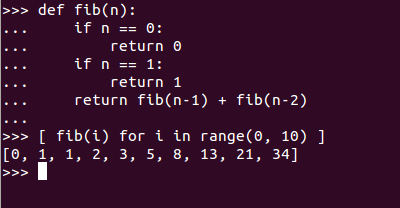
\includegraphics[width=1.0\hsize]{image2012-gum/ipython-pythonshell.png}
      \subfigure{pythonシェル}
      \label{pythonshell}
    \end{minipage}
    \begin{minipage}[b]{0.5\textwidth}
      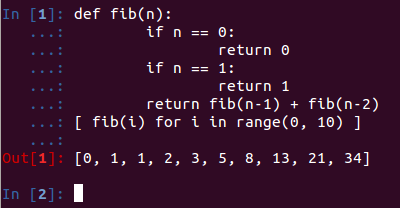
\includegraphics[width=1.0\hsize]{image2012-gum/ipython-terminal.png}
      \subfigure{ipython}
      \label{ipython}
    \end{minipage}
  \end{tabular}
  \caption{pythonシェルとipythonの違い}
\end{figure*}

\subsection{IPython qtconsole}

ipythopnにqtconsoleオプションを指定して実行することにより、
GUI環境でのipythonが起動します。
またこの環境で \texttt{--pylab inline} を指定して起動することで、
コンソール内にグラフを表示させることが可能となります。

\begin{commandline}
$ ipython qtconsole --pylab matplotlib
\end{commandline}

この環境では前述のグラフ表示に加え、
複数行をまとめて扱うコマンドの履歴などが使用できます。
グラフを描画すると次のように表示されます。

\begin{figure}[ht]
  \begin{center}
    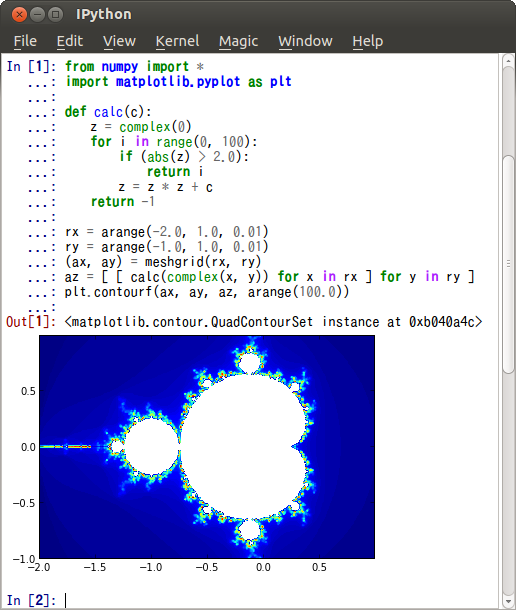
\includegraphics[width=0.6\hsize]{image2012-gum/ipython-mandelbrotset.png}
  \end{center}
  \caption{qtconsoleでマンデルブロ集合}
  \label{fig:ipython-qtconsole}
\end{figure}

testingでのipython qtconsoleおよびmatplotlibは次のコマンドでインストール出来ます。

\begin{commandline}
$ sudo aptitude install ipython-qtconsole python-matplotlib
\end{commandline}

またsqueezeはbackportsを使用してインストールを行いました。
まず/etc/apt/sources.listに次の行を追加し、

\begin{commandline}
deb http://backports.debian.org/debian-backports squeeze-backports main
\end{commandline}

\texttt{aptitude update \&\& aptitude upgrade}を実行した後、
次のコマンドでインストールします。

\begin{commandline}
$ sudo aptitude install python-setuptools python2.6-dev ncurses-dev \
  libzmq-dev python-pygments python-matplotlib pyqt4-dev-tools
\end{commandline}

パッケージのインストール後、
pythonの\texttt{easy\_install}コマンドを使用してipythonをインストールします。

\begin{commandline}
$ sudo easy_install readline pyzmq ipython
\end{commandline}

\subsection{IPython notebook}

ipython notebookはWebベースの数式処理システムで、
次の機能を備えています。

\begin{itemize}
 \item Pythonコードの実行と結果の表示
 \item Markdownによるマークアップ可能なノート
 \item MathJaxによる \TeX 形式での数式の記述
\end{itemize}

\begin{figure}[ht]
  \begin{center}
    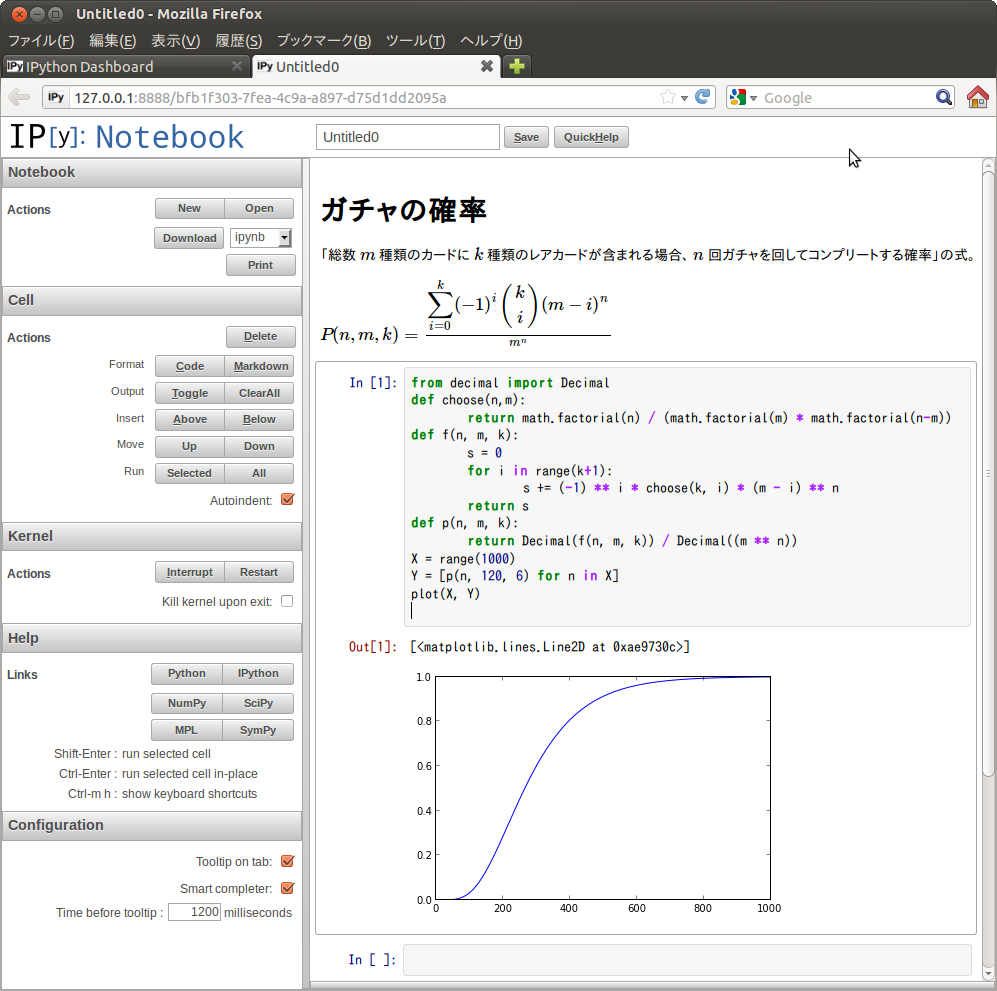
\includegraphics[width=0.80\hsize]{image2012-gum/ipython-gacha.png}
  \end{center}
  \caption{ipython notebookの使用例}
  \label{fig:ipython-gacha}
\end{figure}

testingには次のコマンドでインストール可能です。

\begin{commandline}
$ sudo aptitude install ipython-notebook python-matplotlib python-tornado
\end{commandline}

squeezeはqtconsoleと同様にbackportsを使用します。
ここではsqueezeのiceweaselが古いためこちらもapt lineに追加しています。

\begin{commandline}
deb http://backports.debian.org/debian-backports squeeze-backports main
deb http://mozilla.debian.net/ squeeze-backports iceweasel-release
\end{commandline}

\texttt{aptitude update \&\& aptitude upgrade}を実行した後、
インストールは次のコマンドで行いました。

\begin{commandline}
$ sudo aptitude install python-setuptools python2.6-dev ncurses-dev libzmq-dev python-pygments python-matplotlib
\end{commandline}

パッケージをインストールした後、
pythonの\texttt{easy\_install}コマンドを使用してipythonをインストールします。

\begin{commandline}
$ sudo easy_install readline pyzmq ipython tornado
\end{commandline}

またこのままではMathJaxがCDNを指しているので、
pythonを管理者権限で実行しローカルにインストールします。

\begin{commandline}
from IPython.external.mathjax import install_mathjax
install_mathjax()
\end{commandline}

squeezeのウェブブラウザはどれも古く、
Web Socketの問題からnotebookでは使えません。
そこで最新版のiceweaselを導入します。
ipython notebookは起動時にデフォルトブラウザを起動するため、
導入後はiceweaselをデフォルトブラウザに指定してください。

\begin{commandline}
$ sudo aptitude install -t squeeze-backports iceweasel
\end{commandline}

ipython notebookは次のコマンドで起動します。

\begin{commandline}
$ ipython notebook --pylab inline
\end{commandline}

他のマシンから接続を行う場合、
ブラウザを起動させないためオプション``\texttt{--no-browser}''を、
アクセス許可を与えるためnotebookを起動させるマシンのipアドレスをオプション``\texttt{--ip}''で指定します。

\begin{commandline}
$ ipython notebook --pylab inline --no-browser --ip 192.168.1.40
\end{commandline}

初回起動時には次のような画面が表示されます。

\begin{figure}[ht]
  \begin{center}
    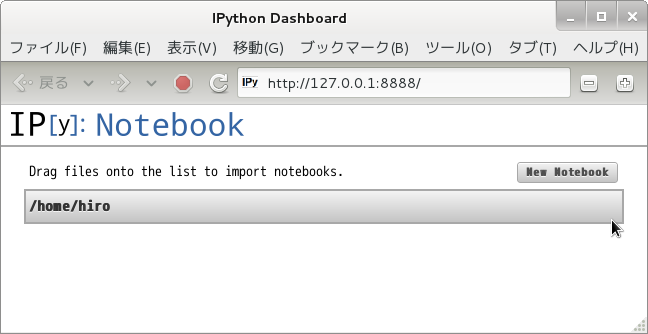
\includegraphics[width=0.67\hsize]{image2012-gum/ipython-notebook.png}
  \end{center}
  \caption{ipython notebookを起動した直後}
  \label{fig:ipython-notebook}
\end{figure}

「New Notebook」ボタンをクリックすることで新規ノートブックが作成され、
空のノートブックがブラウザに表示されます。
MarkdownとPythonのCellは\texttt{Ctrl-m m}および\texttt{Ctrl-m c}で切り替えることができ、
その他コマンドの詳細は\texttt{Ctrl-m h}で表示されます。

作成されたノートブックは表示されているディレクトリ(ここでは/home/hiro/)に``$<$ ノートブックのタイトル$>$.ipynb''というファイル名で保存されます。
このファイルの中身はJSON形式となっています。

\subsection{最後に}

今回はipython qtconsoleおよびnotebookをDebianで使用する方法を紹介しました。
Ubuntu 12.04ではどちらもパッケージとして提供されているため、
wheezyではインストール作業が簡単になると思われます。
これを機会にipythonを活用していただければ幸いです。


%------------------------------------------------------------------------------
\dancersection{DebianとLibreOffice}{あわしろ いくや}
\label{sec:libreoffice}
%------------------------------------------------------------------------------

\subsection{自己紹介}
\subsection{OOoのあらすじ}

\begin{itemize}
\item 1999/8/??…Sun MicrosystemsがStarOfficeの開発企業を買収
\item 2000/10/13…後にOOoとなるソースコード公開
\item 2002/5/1…OOo 1.0リリース
\item 2009/4/20…OracleによるSunの買収を発表
\item 2010/1/27…Oracleによる買収完了
\item 2010/6/4…OOo 3.2.1リリース
\item 2011/1/25…最終バージョンの3.3.0リリース
\end{itemize}

\subsection{LibreOffice その1}

\begin{itemize}
\item 2010/9/28…The Document FoundationとLibreOfficeのリリースを発表
\item OOoのコミュニティメンバーで結成
\item OOoの商標の移譲をOracleに求めてみたり
\item 2011/1/25…LibreOffice 3.3.0リリース
\item 2011/6/3…LibreOffice 3.4.0リリース
\item 2012/2/14…LibreOffice 3.5.0リリース
\item 2012/2/20…TDFが財団に
\end{itemize}

\subsection{LibreOffice その2}
\subsubsection{かなり普通の開発体制になった}

\begin{itemize}
\item ソースコードはgitで管理
\item 契約書にサインしなくてもpushされる
\item ライセンスはLGPLとMPL
\item 毎月リリース、半年に1度メジャーバージョンアップ
\item 今は8月リリースに向けて3.6を開発中
\end{itemize}

\subsection{Apache OpenOffice}

\begin{itemize}
\item 2011/4/15…OracleがOOoの開発中止を発表
\item 2011/4/20…担当社員を全員解雇
\item 2011/6/1…Apacheへの移管を発表
\item 2011/6/13…ApacheのIncubatorプロジェクトに承認
\item 2011/11/17…名称を”Apache Openoffce”に決定
\item 2011/11/31…ライセンスをAL 2に変更する作業完了
\item 2012/5/8…AOO 3.4.0リリース
\item 2012/5/17…AOO 3.4.0 100万ダウンロード
\item 2012/5/21…Lotus Symphonyのコード公開
\item 2012/5/27…AOO 3.4.0 200万ダウンロード
\end{itemize}

\subsection{Apache OpenOffice その2}
\subsubsection{Lotus Symphony}
\begin{itemize}
\item IBMが2008/5/30にリリース
\item OOoとEclipseをベース
\item Sunから特別なライセンス
\item ワープロ・表計算・プレゼン・Webブラウザ
\item Windows/Linuxで動作
\item 無償配布
\item 2012/1/23…最終バージョンの3.0.1リリース
\end{itemize}

\subsection{OOo meets Debian}
\subsubsection{最初のアップロードは2001/10/23}

\begin{itemize}
\item 2002/4/24…0.641d.cvs20020424-1をアップロード
\item 2002/5/1…OOo 1.0リリース
\item 2002/5/2…OOo 1.0 sid入り
\item 2002/7/11…OOo 1.0.1 sid入り
\end{itemize}

\subsubsection{現在のメンテナンス体制}

\begin{itemize}
\item Rene EngelhardさんとBj\"{o}rn Michaelsenさん(Canonical)の二人体制
\item とはいえ、パッケージに関してはReneさんの作業量が多い
\item Bj\"{o}rnさんはupstreamの作業が多い
\item Bj\"{o}rnさんはビルドのスペシャリスト、Reneさんはパッケージングのスペシャリスト
\end{itemize}

\subsection{LibOfficeのパッケージの背景}

\begin{itemize}
\item OOo 3.3.0に関する作業が行われた形跡が全くない
\item 以前はベータ版でも作業が行われていた
\item Reneさんはかなり早い段階からTDFに誘われていたことがわかる
\item 確かにFounderの一人になっている\\
\url{http://www.documentfoundation.org/foundation/history/}
\item その時点でLibOがDebianに入ることは確定的だった
\item LibOがsidで使えるようになったのが2012/2/6
\item 現在でもOpenOffice.orgのパッケージはあるものの、LibreOfficeへの移行用ダミーパッケージ
\end{itemize}

\subsection{LibreOfficeパッケージ}

\subsubsection{libreoffice-3.5.3を例に}

\begin{itemize}
\item ソースを取得後df -hすると3.2GB
\item rulesをwc -lすると3146
\item controlをwc -lすると3380
\item changelogをwc -lすると9763
\item builddでのビルド時間は6時間40分(i386)
\item 必要なディスクスペースは17.04GB
\item パッチはquiltで管理
\end{itemize}

\subsubsection{Debian パッケージの注意点}

\begin{itemize}
\item 得てしてオフィシャルのバイナリを前提とした説明をされる
\item 拡張機能は一切インストールされないので、あとからインストールする。たいていはパッケージ化されている
\item libreoffice-gnome/libreoffice-gtk3/libreoffice-kdeのインストールを忘れない
\end{itemize}

\subsection{LibOffice 関連パッケージ}

\begin{enumerate}
\item ooohg \\
Set of 1600 free of charge maps for libreoffice/openoffice.org
\item openclipart-libreoffice \\
clip art for OpenOffice.org/LibreOffice gallery
\item writer2latex \\
OpenOffice.org Writer/Calc to LaTeX/XHTML converter
\end{enumerate}

\subsection{翻訳のこと}
\subsubsection{皆さんにお願い}
\begin{itemize}
\item \url{discuss@ja.libreoffice.org}を購読してね
\item 翻訳の指摘(誤訳やわかりにくいものなど)
\item 専門的な知識の教示
\item 英語、日本語、ワープロ、表計算(特に関数)、ドロー、Windows、Mac、Linux、数式、データベース、PDF、印刷 etc...
\item 間接的にDebianへの貢献にもなりますよ!
\end{itemize}

\subsection{AOO と Debian}
\subsubsection{6月上旬現在、パッケージなし}
\begin{itemize}
\item 怪しいリポジトリはある\\
\url{http://apacheoo-deb.sourceforge.net/}
\item オフィシャルビルドのDebパッケージをaptで取れるようにしているだけ
\item ちなみにlaunchpadにプロジェクトはあるけどパッケージはない\\
\url{https://launchpad.net/~apacheopenoffice}
\end{itemize}

\subsubsection{オフィシャルビルドのDebパッケージ}
\begin{itemize}
\item EPMで生成
\begin{itemize}
\item ESP Package Manager
\item これはLibreOfficeも一緒
\item 原作者はCUPSの作者
\item RPMとかDebパッケージを生成するもの
\item すなわち、debianフォルダがあるわけじゃない
\item どうやってもオフィシャルにならない
\end{itemize}
\end{itemize}
\subsubsection{3月にdebian-usersとdebian-openofficeでAOOに関する投稿あり}
\begin{itemize}
\item \url{http://lists.debian.org/debian-user/2012/03/msg00824.html}
\item \url{http://lists.debian.org/debian-openoffice/2012/03/msg00103.html}
\end{itemize}
いずれもReneさんが激しく拒否

\subsection{さらなる情報}
\subsubsection{主に歴史を知りたい人向け}
\begin{enumerate}
\item 2011年のOpenOffice.org/LibreOffice
\\
\url{http://gihyo.jp/lifestyle/column/newyear/2011/openoffice-prospect}
\item LibreOffice/Apache OpenOffice 〜2011年の総括と新たな選択〜
\\
\url{http://gihyo.jp/lifestyle/column/newyear/2012/libreoffice-prospect}
\end{enumerate}

%------------------------------------------------------------------------------
\dancersection{debug.debian.net}{岩松 信洋}
\label{sec:debug.debian.net}
%------------------------------------------------------------------------------

\subsection{はじめに}
現在、Debian Project で配布されているパッケージでは、
デバッグ情報が削除された状態で配布されています。
この理由として、デバッグ情報はほとんどのユーザには必要ないものであるという点と、
デバッグ情報を保持している実行ファイルはサイズが非常に大きいため、ディスクを圧迫
するという点があります。
しかし、デバッグ情報があるとデバッグを行うときにとても有用な情報となりいろいろと便利です。
今回、Debian で全てのDebianパッケージにおいてデバッグ情報を提供する方法を考えて実装してみま
した。その課程と今後について説明します、

\subsection{Debug情報とDebianパッケージ}
Debian はバイナリベースディストリビューションの一つです。
基本的に配布されているパッケージではデバッグ情報が削除された状態で配布されています。
このデバッグ情報は、内部シンボルや型の情報、ソースコードの行番号などを指します。

実行ファイルのデバッグ情報がある場合、以下のようなよい点があります。
\begin{itemize}
\item デバッガ(GDB)を使ったデバッグでより詳細なデバッグ情報を得ること
ができる
\item デバッグ情報を含めたバイナリを再度ビルドする必要がない
\item バイナリベースディストリビューションの場合、実際のバイナリとデバッグ情報が常に
対になるので、バグの再現性が高くなる
\end{itemize}
%これらは組み込み用途にもよく利用されているDebianでは特に有効に働きます。
%また、デバッグ情報を含めるためのパッケージ作成方法(DEB_BUILD_OPTIONS=nostrip をを環境
%変数にエクスポートする)を調べる必要もありません。

逆に悪い点として以下のようなものがあります。

\begin{itemize}
\item 実行ファイルにデバッグ情報が含まれるので実行ファイルのサイズが大きくなる
\item デバッグしない人にとっては不要なものが含まれることになる
\end{itemize}

これらをまとめると、すべての実行ファイルのデバッグ情報が提供されており
ユーザにとって必要のない情報がインストールされない仕組みがあれば
デバッグ情報はとても有益なものになるはずです。
Debian ではいくつかのソースパッケージからデバッグ情報を含んだパッケージが提供されています。
このパッケージには\texttt{-dbg} というサフィックスが付いてます。
特にデバッグ情報用のパッケージに関するポリシーは決まっておらず、提供に関してはパッケージメンテナ
次第という状態になっています。今まで提供されなかった理由としてはディスク容量の問題や回線の
問題等があったようですが、個人的に今は特に問題はないと思っています。

ちなみに、Fedoraでは \texttt{-debuginfo} というサフィックスを持ったパッケージが提供されており、
Gentooではデフォルトでこれらの情報を生成し管理しています。このようにデバッグ情報の提供という点に
関して他のディストリビューションに遅れを取っています。

\subsection{Debianでのデバッグ情報パッケージについて}
まず、実装した内容について説明する前に今のデバッグ情報パッケージの提供方法について説明します。
Debianではデバッグ情報パッケージは \texttt{-dbg} というサフィックスがついたパッケージ名を持ちます。
例えば foo というアーキテクチャ依存のパッケージがあった場合、\texttt{foo} のデバッグ情報を持ったパッケージ名は
\texttt{foo-dbg} になります。
そして、Debian の \texttt{-dbg} パッケージで提供されているバイナリは動作するバイナリデータではなく、
デバッグ情報のみを持ったデータになっています。 このファイルは \texttt{objdump --only-keep-debug}
を実行することによって生成することができます。もちろん対象の実行ファイルはコンパイル時にデバッグ情報
が付加されている必要があります。
その後、デバッグ情報ファイルへのリンクを \texttt{strip} 済の実行可能形式に付加するために
\texttt{objcopy --add-gnu-debuglink} を実行します。
これによって、実行ファイルとデバッグ情報ファイルが対になります。
GDB を使ってデバッグする際には実行ファイルとデバッグ情報ファイルはリンク
しているので、デバッグ情報ファイルがインストールされているときは自動的に呼ばれ、デバッグ
シンボルなどを読み込んでくれます。

\subsection{実装について}

先に説明したようにに、すべての実行ファイルのデバッグ情報が提供されており
ユーザにとって必要のない情報がインストールされない仕組みがあればよいので、
これらに対応できる方法を考えました。以下で説明します。

\subsubsection{すべての実行ファイルのデバッグ情報を提供する}
すべての実行ファイルのデバッグ情報を提供するには、全てのパッケージで
\texttt{strip} された実行ファイルとデバッグ情報ファイルを持ったパッケージを構築すれば
よいわけです。


Debian の場合、パッケージはデバッグ情報が有効な状態(\texttt{gcc} だと\texttt{-g} オプション等)
でビルドされます。そしてパッケージにされる時に \texttt{strip} (binutilsに含まれる)
が \texttt{dh\_strip} から呼ばれ、実行ファイルやライブラリならデバッグ情報が削除され、
パッケージ用のディレクトリにコピーされ、\texttt{dh\_builddeb} コマンドでパッケージ化されます。

そして、配布される -dbg パッケージは \texttt{dh\_strip}を実行するときにデバッグ情報を提供する
パッケージとして、\texttt{dh\_strip} のオプションとして指定されるか、debian/control ファイルに列挙されている
パッケージ名のサフィックに \texttt{-dbg} が付いている場合、対象ファイルとして処理されます。

ここ問題なのが、
\begin{enumerate}
\item 自動生成したい デバッグ情報パッケージ情報をどのように生成するか
\item \texttt{dh\_strip} でデバッグ情報パッケージ指定されている場合、自動生成したい -dbg パッケージ用のファイルを
どのように生成するか
\item 自動生成したいデバッグ情報パッケージそのものをどのように生成するか
\end{enumerate}
という点です。

問題点1についての対処方法ですが、\texttt{dh\_strip} の処理の先頭で debian/control ファイルに
デバッグ情報パッケージファイルに関する情報を追記する処理を追加しました。
デバッグ情報パッケージはそのパッケージがアーキテクチャ依存(Architechture: all ではない)
事とパッケージ名さえわかれば、パッケージ情報は自動生成できます。
例えば、\texttt{hoge} というパッケージがあってデバッグ情報パッケージが提供されていない場合、
以下のような内容を追記します。

\begin{commandline}
Package: hoge-dbg
Architecture: any
Section: debug
Priority: extra
Depends: hoge (= \${binary:Version}), \${misc:Depends}
Description: debugging symbols for hoge
 This package contains the debugging symbols for hoge
\end{commandline}

次に問題点2の対処方法ですが、アーキテクチャ依存のDebianパッケージは \texttt{dh\_strip} が呼ばれるため、ここで
処理をフックしてしまえば、デバッグ情報を提供するパッケージと用のデータと \texttt{strip} された
バイナリデータを分けることができます。今回は \texttt{dh\_strip} の中身を改造し、全てのアーキテクチャ依存の
パッケージ用のデータを作成することにしました。\texttt{dh\_strip}でパッケージが指定されていても
それを無視するように処理を変更するだけです。

問題点3の対処方法ですが、デバッグ情報パッケージは \texttt{dh\_strip} 内で \texttt{dh\_builddeb} を呼び出すことで
対応しました。パッケージ名とパッケージ作成に必要なデータは揃っているので、
\texttt{dh\_builddeb -pデバッグ情報パッケージ名} を実行することで、パッケージが作成されます。

これらが行える前提条件として、debhelper に依存しているパッケージが対象になります。
現在ほとんどのパッケージが debhelper か CDBS に依存しており、CDBS は debhelper と
同時に使う事が多いため(実際、CDBSに依存しているパッケージは全てdebhelper に依存しています。dbsも同様です。)
問題ではありません。
\footnote{\url{http://people.debian.org/~cjwatson/dhstats.png}}

\subsection{パッケージサイズへの対応}

次にパッケージサイズの問題です。
デバッグ情報は非常に大きく、\texttt{strip} されたバイナリの数倍以上のサイズになることは
めずらしくありません。例えば libjpeg8 で提供される libjpeg.so.8.4.0 のファイル
サイズは表\ref{tab:debuginfo-jpegsize}となりました。

\begin{table}[ht]
 \caption{libjpeg.so.8.4.0 各状態のファイルサイズ}
 \label{tab:debuginfo-jpegsize}
\begin{center}
  \begin{tabular}{|c|c|}
 \hline
 状態 & サイズ \\
 \hline
 strip 前 & 約1.3MB \\
 strip 後 & 236KB \\
 デバッグ情報ファイル & 1.1MB \\
 \hline
 \end{tabular}
\end{center}
\end{table}

このようにサイズが大きく異なるので、パッケージを分けてもユーザが利用しているパッケージリポジトリ
と同じ場所・方法で提供してしまうと、ミラーに時間がかかるようになりますしユーザに不要なデータが格納されたリ
ポジトリ情報を持たせるようになります。

今回、この問題を回避するためにリポジトリを分けることを考えました。
例えば、unstable で \texttt{strip} されているパッケージ(通常のパッケージ)は unstable とだけ指定し、
デバッグ情報を提供するパッケージは unstable/debug するという方法です。
例を図\ref{fig:debuginfo-apt-line}に示します。

\begin{figure}[ht]
\begin{center}
\begin{commandline}
deb http://cdn.debian.or.jp/debian/ unstable main non-free
deb http://cdn.debian.or.jp/debian/ unstable/debug main
\end{commandline}
\end{center}
 \caption{デバッグ情報パッケージを利用する場合の apt-line 設定例}
 \label{fig:debuginfo-apt-line}
\end{figure}


デバッグ情報が必要なユーザは unstable/debug を apt-line に追加することによってデバッグ情報
用のパッケージが利用できるようになります。
またパッケージが格納されるディレクトリのパスを変更することによって、デバッグ情報のみを
提供するミラーを構築することができ、debug 情報をミラーしないミラーサーバの負荷も今までと変わ
らないという事になります。

\subsubsection{実装後について}

これらを実装したシステムを reprepro + sbuild + rebuildd で構築しました。
現在stable/amd64のみをターゲットテストとして動作させています。
まだ全てビルドできていません。さくらのVPSで1週間ほどビルドしていますが、
まだgnome-power-managerをビルドしているところで、進捗率は40\%といったところでしょうか。

\subsection{考えられる問題}

\subsubsection{セキュリティの問題}
現在、ソースパッケージから作成されたバイナリバッケージの一覧は .changesファイルに
ファイルのハッシュと共に記述され、どのソースパッケージ(orig.tar.gz, dsc.diff.gz)
から作成されたのか分かるようになっています。
現時点での実装はバイナリパッケージ作成の課程で自動生成されるためのこれらの情報
とリンクしません。Buildd上でデバッグ情報ファイルパッケージが生成されるので個人的に
問題ないと思っていますが、これらを紐付けるシステムがあるほうがより安全と言えるでしょう。

\subsubsection{バイナリの不一致}
既存のシステムだと、\texttt{strip} されたバイナリと デバッグ情報が一致しないので
オフィシャルのバイナリと混ぜて使えないことが考えられます。私が提供している
されているデバッグ情報パッケージを使う場合、
私が提供してる通常のパッケージも利用しないと意味がないでしょう。
今はこれをバージョンによる依存関係で回避しています。
最終的には buildd に入れてもらうことでデバッグ情報パッケージを自動生成することを
考えています。

\subsection{そもそも debug.debian.netがあるんじゃね?という話}
さて、私のような凡人が考えるようなことは先人達はすでに考えているわけでして、
(既に行なっていることを知ったのは大統一勉強会スケジュールが出てからなのですが。)
既に \url{http://debug.debian.net}というサービスがあり実装され、そして終了していました。
実装と考えもほとんど同じです。大きく違うところはデバッグ情報パッケージの
サフィックスが\texttt{-dbg}ではなく、\texttt{-dbgsym}である点と、
デバッグ情報を作成する部分が \texttt{dh\_builddeb} ではなく、\texttt{dpkg-deb} を使っている
点、そして\texttt{dh\_strip}を直接変更するのではなく、シンボリックリンクで
機能をオーバーライドさせている点です。こちらの方がdebhelperに手を加えなくて済むので
こちらに乗り換えて、いくつかの修正を行いました。
元々このサービスは myon \footnote{Christoph Berg氏。DAM の一人。} がやっていたのですが、
彼に連絡を取り、再稼働させることにしました。この発表が行われている頃には稼働していると思います。

\subsection{今後の課題}

このままスタンドアロンでデバッグ情報パッケージを提供しても無駄なバイナリを生成するだけなので、
buildd にこのシステムを入れてもらい、dak で ディストリビューション/debug として
処理してもらうことが今後の大きな課題になっています。このことについて来月開催される Debconf 12
でBOF またはFTPチーム、wanna-builddチームと話ができればと思っています。

\subsection{最後に}
アーキテクチャに依存している Debian パッケージでデバッグ情報を
パッケージとして提供する方法について説明しました。文中ではユーザには
あまり必要のない機構のように取り扱いましたが、バグレポートをする際、
デバッグ情報があるとより内容の濃いバグレポートを提出できるようになり、
開発者を手助けできるようになります。この機構が正式採用された時に、
自分が使っているパッケージのデバッグ情報パッケージだけでもインストール
してくれれば幸いです。

%------------------------------------------------------------------------------
\dancersection{Rabbit: 時間内に終われるプレゼンツール}{須藤功平}
\label{sec:Rabbit}
%------------------------------------------------------------------------------

% add upper space for logo
\vspace{2em}

Debian GNU/Linux上で動作するプレゼンテーションツールRabbitを紹介します。
まず、Rabbitの代表的な機能である時間内に終われるための機能を紹介し、そ
の後、Debian GNU/Linux上でRabbitをインストールする方法とスライドを作る
方法を簡単に紹介します。

\subsection{Rabbitとは}

RabbitはRubyとGTK+で実装されたプレゼンテーションツールです。Debian
GNU/Linuxを含む多くのプラットフォーム上で動作します。

Debian GNU/Linux上で動作するプレゼンテーションツールはたくさんあります。

\begin{itemize}
\item GUIでスライドを作成するデスクトップアプリケーション
  (LibreOfficeのImpressなど)
\item テキストで作成したスライドを表示するデスクトップアプリケーション
  (MagicPointやRabbitなど)
\item \LaTeX{}のBeamerクラス + PDFビューアー(Evinceやpdfcubeなど)
\item JavaScript + Webブラウザ(Impress.jsやshowoffなど)
\item Webサービス(Google DocsやPreziなど)
\end{itemize}

それぞれのツールは特徴が大きく異なっており、それぞれよいところがありま
す。Rabbitにもまた特徴があり、他のツールにはない便利な機能があります。
それが「プレゼンテーションを時間内に終われるための機能」です。この機能
は一般的にタイマー機能と呼ばれているもので、プレゼンテーション中に残り
時間を表示して、発表者に進み具合を伝える機能です。多くのツールでこの機
能を提供していますが、Rabbitのタイマー機能はどう違うのでしょうか。一言
でいうとUI(ユーザーインターフェイス。見た目)が違います。他は同じで
す。

\subsubsection{RabbitのUI}

タイマー機能はMagicPointも提供していますし、Impressも提供しています。
図\ref{fig:normal-timer-ui}のように、MagicPointはスライド下部にとても目
立たないように緑のバーを表示します。Impressはスライド表示用のモニターと
は別のモニターに経過時間を表示します。このように発表者にだけわかるよう
に表示するUIが一般的なタイマー機能のUIです。

\begin{figure}[ht]
  \begin{center}
    
\includegraphics[width=1\hsize]{image2012-gum/normal-timer-ui.eps}
  \end{center}
  \caption{従来のタイマー機能のUI}
  \label{fig:normal-timer-ui}
\end{figure}

一方、RabbitのUIは発表者だけではなく観客にもわかりやすく表示します。
図\ref{fig:rabbit-timer-ui}のように、スライド下部にうさぎとかめを表示し
ます。それも誰が見ても気づくくらいの大きさで表示します。このようにタイ
マー機能を観客からもわかりやすく表示するUIは既存のプレゼンテーションツー
ルとは一線を画します。

\begin{figure}[ht]
  \begin{center}
    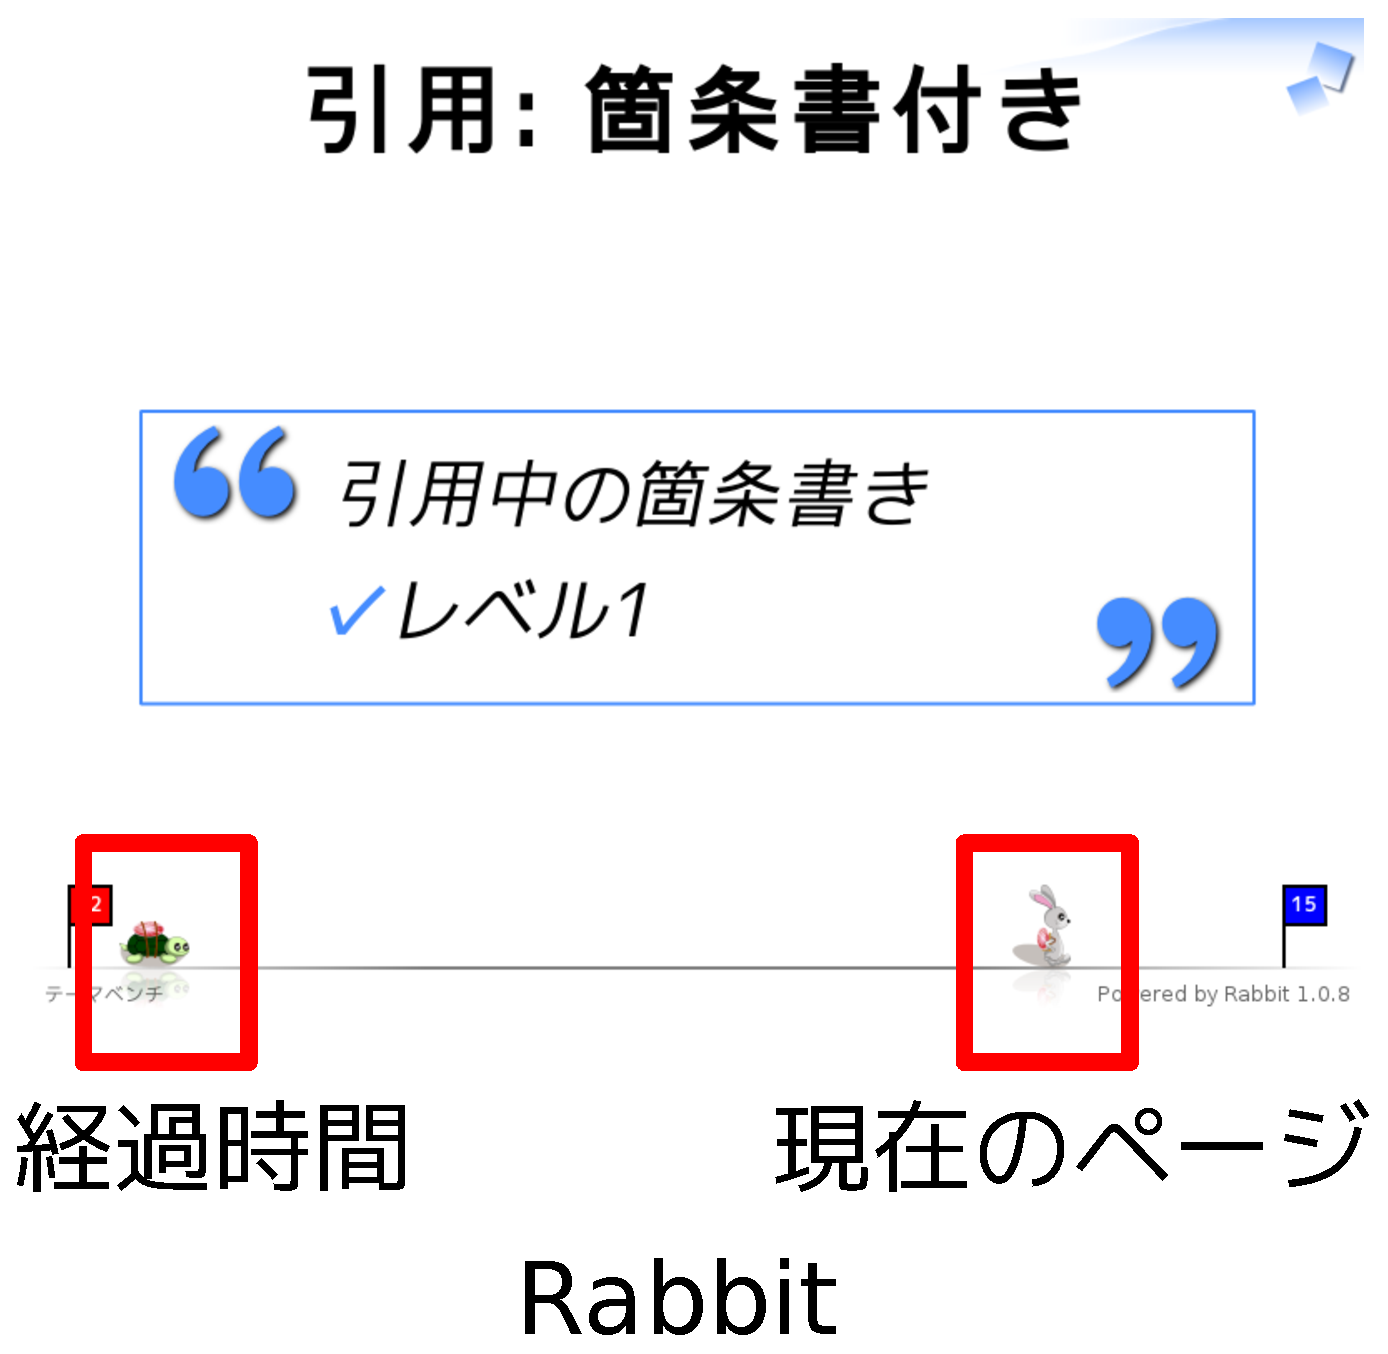
\includegraphics[width=0.5\hsize]{image2012-gum/rabbit-timer-ui.eps}
  \end{center}
  \caption{Rabbitのタイマー機能のUI}
  \label{fig:rabbit-timer-ui}
\end{figure}

それでは、このUIがどうして時間内に終わるための効果を提供するかを考えて
みましょう。

\subsubsection{みんなにわかるUI}

このRabbitのUIの特徴は発表者だけではなく、観客にも発表の進み具合がわか
りやすいという点です。発表時間を過ぎれば経過時間を表しているかめが画面
の右側に走りすぎていきます。もちろん、かめなので徐々に画面の右側に進ん
でいきます。そのため、観客が気づかないうちに発表時間を過ぎていたという
ことは起きません。発表時間を過ぎても終わらないと、たとえどれだけ魅力的
な話であっても気まずい空気になってきます\footnote{要出典。}。

発表者は観客の反応がよいとよりすばらしい発表ができますが、逆に反応が悪
いと、準備してきた成果を発揮しづらいものです。発表時間が過ぎても終わら
ない場合、観客の反応が悪くなります。この状態でさらに続けることはとても
つらいため自然と終わらせようという力が働きます。

このように、タイマー機能を発表者だけではなく観客からもわかりやすいUIに
することにより、観客から残り時間に関するフィードバックを受け取ることが
できます。発表者が残り時間を意識するだけではなく、観客からのフィードバッ
クもあわせることで自然と時間内に終われる発表になります。ただし、観客に
わかりやすいタイマー機能のUIなので、発表内容よりもうさぎとかめの競争に
集中してしまい、肝心の発表内容に集中してもらえないという危険性がありま
す。時間内に終わることだけではなく、魅力的な発表内容を用意することにも
十分注意してください。

\subsection{インストール方法}

ここまでの紹介でRabbitを使いたくなっているはずです。ここからはRabbitの
使い方を紹介します。

まず、RabbitをDebian GNU/Linuxへインストールする方法を紹介します。イン
ストール方法は2種類あります。

\begin{itemize}
\item aptを使う
\item RubyGemsを使う
\end{itemize}

最新バージョンを使いたい場合やフル機能を使いたい場合はRubyGemsを使う方
法がオススメです。簡単にインストールしたい場合はaptを使う方法がオススメ
です。

\subsubsection{aptでインストール}

1つ目の方法は、aptを使う方法です。Rabbitのdebパッケージは公式aptリポジ
トリに含まれている\footnote{大統一Debian勉強会の実行委員でもある佐々木
  洋平さんがパッケージメンテナー。}ので以下のようにすれば簡単にインストー
ルできます。

\begin{commandline}
$ sudo apt-get -V -y install rabbit
\end{commandline}
%$
以下のコマンドを実行してスライドが表示されたら正常にインストールできています。

\begin{commandline}
$ rabbit https://raw.github.com/shockers/rabbit/master/sample/theme-bench.rab
\end{commandline}
%$
\subsubsection{RubyGemsでインストール}

2つ目の方法はRubyGemsを使う方法です。RabbitはGTK+などたくさんのライブラ
リを利用しています。そのため、まず、関連ライブラリをaptでインストールし
ます。

\begin{commandline}
$ sudo apt-get -V -y install \
    ruby1.9.1 ruby1.9.1-dev libgtk2.0-dev librsvg2-dev libpoppler-glib-dev \
    libxml2-dev libxslt1-dev
\end{commandline}
%$

関連ライブラリをインストールしたらRubyGemsでRabbitをインストールします。

\begin{commandline}
$ sudo gem1.9.1 install rabbit twitter-stream twitter_oauth
\end{commandline}
%$

以下のコマンドを実行してスライドが表示されたら正常にインストールできています。

\begin{commandline}
$ PATH="/var/lib/gems/1.9.1/bin:$PATH"
$ rabbit https://raw.github.com/shockers/rabbit/master/sample/theme-bench.rab
\end{commandline}
%$
\subsection{スライドの作り方}

Rabbitを使う準備ができたので自分でスライドを作る方法を紹介します。

RabbitはMagicPointのようにテキストでスライドを作成します。テキストの
フォーマットにはRD\footnote{Ruby Documentの略。}やWiki形式、Markdownな
どいくつもの有名なフォーマットをサポートしています。ここでは、RDでのス
ライドの書き方を紹介します。

\subsubsection{RDでのスライドの作り方}

RDでスライドを作る場合、以下のように「{\tt{=}}」でスライドを区切ります。
「{\tt{=}}」の行に書いているテキストがそのスライドのタイトルになります。
「{\tt{\#}}」から始まる行はコメントです。シンプルですね。

\begin{commandline}
# slide.rab

= タイトルスライド

# 持ち時間
: allotted-time
   5m

= 最初のスライド

  * 1枚目のスライドの内容

= 2枚目のスライド

  * 2枚目のスライドの内容
\end{commandline}

最初のスライドは特別でタイトルスライドになります。ここにはスライド全体
のメタデータを指定することができます。「{\tt{allotted-time}}」というのは
このプレゼンテーションの持ち時間で、「{\tt{5m}}」は5分\footnote{5
  Minutes}という意味です。持ち時間を指定するとうさぎとかめタイマーが表
示されるので、持ち時間が決まっているプレゼンテーションのときは指定しま
しょう。

作成したスライドは以下のように実行します。2ページ目を表示するとうさぎと
かめタイマーが動きだします。

\begin{commandline}
$ rabbit slide.rab
\end{commandline}

\subsubsection{PDFで作成したスライドの表示方法}

Rabbitはスライドを表示する機能だけを提供しているため、スライド作成を支
援する機能はありません。Debian GNU/Linuxを使っている人はエディターでテ
キストを編集することに慣れているでしょうが、たまにはImpressなどを使っ
てGUIでグラフィカルにスライドを作成したくなるかもしれません。そのときは
そのようなツールでスライドを作成してください。Rabbitはテキストだけでは
なくPDFファイルも読むこむことができます。Impressなどでスライドを作成
しPDFで出力すれば、Rabbitで表示することができます。

PDFを表示するときはコマンドラインから持ち時間を指定します。
「{\tt{--allotted-time 5m}}」と指定すると持ち時間が5分という意味になりま
す。2ページ目を表示するとうさぎとかめタイマーが動きだします。

\begin{commandline}
$ rabbit --allotted-time 5m slide.pdf
\end{commandline}

\subsection{さいごに}

Debian GNU/Linux上で動作する時間内に終われるプレゼンテーションツー
ルRabbitを紹介しました。Debian GNU/Linuxでプレゼンテーションをする人た
ちの参考になることを期待しています。

もっとRabbitを知りたくなった人は公式サイ
ト\url{http://rabbit-shockers.org/}をのぞいてみてください。

%------------------------------------------------------------------------------
\dancersection{U-Bootについてあれこれ}{野島 貴英}
\label{sec:u-boot-arekore}
%------------------------------------------------------------------------------

\vspace{2em}
% Add upper space for logo

Debianは組み込み用途の開発にも非常に便利の良い開発環境を作る事ができます。
ここでは、組み込み用途の開発では最も基本的なソフトウェアであるブートローダ
をDebianの環境を用いてU-Bootを用いて開発してみます。最後に、電子書籍端末に
ブートローダを実際に搭載して起動を試みます。

\subsection{U-Bootとは}

U-Bootとは、DENX Software Engineering社(本家)で主にメンテされている
ブートローダです。Das U-Bootともいう\footnote{ドイツ語で潜水艦の意。この場合直訳すると「ザ・潜水艦」と言う感じです。}そうです。

元はPowerPC用途のブートローダだった模様ですが、様々な人が拡張を加え、現在では216種類の組み込み機材に対応しており、さらに対応数は増えつづけてている模様です\cite{u-boothistory}。

\subsection{U-Bootの特徴}

以下に示す沢山の特徴があります。

\begin{itemize}
\item ソフトウェアライセンスはGPL v2です
\item 沢山のCPU、組み込み機材に対応しています。例:PowerPC,ARM,AVR32,Blackfin,m68k,x86,...
\item U-Bootのソース本体は単機能の部品の塊であり、ディレクトリも十分に整理され、マクロも整理されている為、開発対象の機材に合わせた改造をするにも、直感的で非常にわかりやすいです
\item U-Boot独自仕様のちょっとしたスクリプト言語を使う事により、ブートに関して機材に合わせた制御が可能です。また、対話的にOSをブートさせる事ができます
\item tftp経由のOSブート、シリアル経由のOSブート、NFS経由のOSブート、数々の種類のFlashメモリからのOSブート等、様々な方法でOSをブートすることが可能です
\item OSイメージを様々な形式のファイルシステム上に置いて起動させることができます。例:fat/vfat形式、ext2/3形式、cramfs形式
\item ELF/バイナリ形式/圧縮形式で出来ているOSのイメージに対応しています
\end{itemize}

\subsection{試しにDebian上で動かしてみる}

まず、Intel 64bit対応版 Debian sidの動作するPCを用意します。

ここで、端末を開き(端末A)、experimental版のQEMUを導入します。

\begin{commandline}
端末A $ cat /etc/apt/sources.list
deb http://ftp.jp.debian.org/debian/ sid main contrib non-free
deb-src http://ftp.jp.debian.org/debian/ sid main contrib non-free
deb http://ftp.jp.debian.org/debian/ experimental main contrib non-free
deb-src http://ftp.jp.debian.org/debian/ experimental main contrib non-free
端末A $ sudo apt-get update
端末A $ sudo apt-get install qemu-system/experimental  <--experimental版導入
\end{commandline}
%$
次にARM用のクロスコンパイル環境を用意します。ここではEmdebianを利用
することにします。なお、現在、Emdebianのパッケージは安定版のDebianでないと
導入ができないものが多い(特にgcc)ため、クロスコンパイル環境として安定版の
Debianのchroot環境を用意して導入することにします。

\begin{commandline}
端末A $ mkdir cross-compile
端末A $ sudo debootstrap --arch amd64 --include emdebian-archive-keyring,\
        sudo,lv,build-essential,binutils-multiarch squeeze \
        `pwd`/cross-compile http://ftp.jp.debian.org/debian
 ...しばらく待つ...
端末A $ env LANG=C sudo chroot `pwd`/cross-compile /bin/bash
(ここからは安定版のDebianとなる)
端末A # echo 'deb http://www.emdebian.org/debian/ squeeze main' >> /etc/apt/sources.list
端末A # echo 'deb-src http://www.emdebian.org/debian/ squeeze main' >> /etc/apt/sources.list
端末A # apt-get update
端末A # groupadd -g <your-gid> <your-id>
端末A # useradd -m -s /bin/bash -u <your-uid> -g <your-gid> -c 'your name' <your-id>
端末A # passwd <your-id>
端末A # echo '127.0.0.1  localhost <your-hostname>' > /etc/hosts
端末A # echo '<your-id> ALL=(ALL) NOPASSWD: ALL' > /etc/sudoers.d/<your-id>
端末A # chmod 440 /etc/sudoers.d/<your-id>
端末A # su - <your-id>
端末A % sudo apt-get install gcc-4.4-arm-linux-gnueabi
\end{commandline}
%$

次に別の端末(端末B)をsid側で開き、u-bootのソースコードを端末Aのディレクトリへ
直接ダウンロードします。

\begin{commandline}
端末B $ cd cross-compile/home/<your-id>/u-boot
端末B $ apt-get source u-boot <---unstable版のu-bootのソースがダウンロードされる。
\end{commandline}

端末AにてARM versatilepb QEMU用にクロスコンパイルします \footnote{versatilepb用のu-boot.binイメージはDebianではパッケージ化されていません}。

\begin{commandline}
端末A $ cd u-boot/u-boot-2012.04.01
端末A $ make ARCH=arm CROSS_COMPILE=arm-linux-gnueabi- versatileqemu_config
端末A $ make ARCH=arm CROSS_COMPILE=arm-linux-gnueabi-
\end{commandline}
%$
出来上がったu-boot.binを端末Bにて、QEMUを使ってARM versatilepb環境で
動作させます\cite{qemu-u-boot}。

\begin{commandline}
端末B $ qemu-system-arm -M versatilepb -nographic -kernel u-boot.bin

U-Boot 2012.04.01 (Jun 05 2012 - 22:34:41)

DRAM:  128 MiB
WARNING: Caches not enabled
Using default environment

In:    serial
Out:   serial
Err:   serial
Net:   SMC91111-0

VersatilePB # printenv
baudrate=38400
...中略...
\end{commandline}
%$

無事U-Bootが動作しています。U-Bootのコマンドラインをいろいろいじってみると
色々分かってよいかと思います。もちろんですが、\$(src)/include/configs/versatile.hや、\$(src)/boards/armltd/verrsatile以下をいじってみていろいろ試すのも非常に簡単に
できてしまいますので、大変おすすめです。

\subsection{実機で動かしてみる}

実機として、Barnes \& Noble社(以下B\&N社)のNook Color端末を使います。

\subsubsection{下準備}

\label{sec:u-boot-sitajunbi}
東京エリアDebian勉強会2012年4月資料の「Android機でDebian」を参照して、
B\&N社のNook Color端末でブート可能なmini-SDカードを作成
しておきます\cite{android-debian}。

B\&N社より配布されているU-Bootのソースに簡単なパッチを当てて、U-Bootのprintf()などがLCDへ表示が出来るようにしてしまいます。また、ついでに、LCDのテストということでカラーバーを表示するようにしてしまいます。

※先ほどの端末A、端末Bを環境として使います。

\begin{commandline}
端末B $ cat u-boot-nook-patch.patch
diff -ru u-boot/common/lcd.c u-boot-nozzy/common/lcd.c
--- u-boot/common/lcd.c 2011-04-20 19:19:16.000000000 +0000
+++ u-boot-nozzy/common/lcd.c   2012-06-05 18:26:47.000000000 +0000
@@ -363,11 +363,11 @@

        strcpy (lcddev.name, "lcd");
        lcddev.ext   = 0;                       /* No extensions */
-#ifdef CONFIG_3621EVT1A
-    lcddev.flags = 0; /* Use only for splash */
-#else
+// #ifdef CONFIG_3621EVT1A
+//    lcddev.flags = 0; /* Use only for splash */
+// #else
        lcddev.flags = DEV_FLAGS_OUTPUT;        /* Output only */
-#endif
+// #endif
        lcddev.putc  = lcd_putc;                /* 'putc' function */
        lcddev.puts  = lcd_puts;                /* 'puts' function */

diff -ru u-boot/include/configs/omap3621_evt1a.h u-boot-nozzy/include/configs/om
ap3621_evt1a.h
--- u-boot/include/configs/omap3621_evt1a.h     2011-04-20 19:19:16.000000000 +0
000
+++ u-boot-nozzy/include/configs/omap3621_evt1a.h       2012-06-05 19:15:52.0000
00000 +0000
@@ -211,6 +211,12 @@
 // Recovery mode boot commands
 //  androidboot.hardware=omapzoom2
 #define CONFIG_EXTRA_ENV_SETTINGS              \
+"stdout=lcd" \
+       "\0" \
+\
+"stderr=lcd" \
+       "\0" \
+\
 "mmcbootdev=0" \
        "\0" \
 \
@@ -556,7 +562,11 @@
 /* Enable LCD driver support for Encore device */
 #define CONFIG_LCD  1
 #define CONFIG_LCD_LOGO 1
-#define CONFIG_LCD_NOT_ENABLED_AT_INIT
+// #define CONFIG_LCD_NOT_ENABLED_AT_INIT
+#define LCD_TEST_PATTERN
+
+/* enable console to lcd */
+#define CFG_CONSOLE_IS_IN_ENV

 /* define early driver board init to allow board initialization after i2c*/
 #define CONFIG_DRV_BOARD_INIT 1
\end{commandline}

上のパッチをあてます。

\begin{commandline}
端末B $ wget http://images.barnesandnoble.com/PResources/download/Nook/source-code/nookcolor_1.4.tgz
端末B $ tar xzf nookcolor_1.4.tgz
端末B $ cd nookcolor-1.4/distro/u-boot
端末B $ patch -p1 < ../../../u-boot-nook-patch.patch
\end{commandline}
%$

パッチをあてたU-Bootのソースをクロスコンパイルしてu-boot.binを作ります\cite{orig-kernel-nook}。

\begin{commandline}
端末A $ cd nookcolor-1.4/distro/u-boot
端末A $ make -j2 ARCH=arm  CROSS_COMPILE=arm-linux-gnueabi- omap3621_evt1a_config
端末A $ make -j2 ARCH=arm  CROSS_COMPILE=arm-linux-gnueabi-
\end{commandline}
%$

出来たu-boot.binを\ref{sec:u-boot-sitajunbi}章で作成しておいたmini-SD上の
u-boot.binと入れ替えます。これで準備完了です。

\subsubsection{起動する}

いよいよmini-SDをNook Color端末に挿入し、電源ボタンを長押しします。
無事、図\ref{fig:u-boot-booting}のとおりU-Bootの起動画面がLCDに出ました。

\begin{figure}[ht]
  \begin{center}
    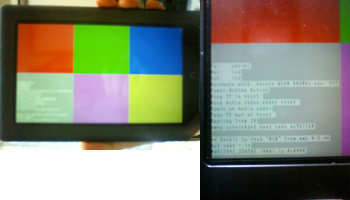
\includegraphics[width=1\hsize]{image2012-gum/u-boot-nook.png}
  \end{center}
  \caption{U-Bootが起動している様子}
  \label{fig:u-boot-booting}
\end{figure}

なお、ここで紹介するU-Bootの改造は、まだ不十分なため、続くuImageをmini-SDから
ロードしてカーネルを実際に立ち上げるところまでは出来ていません。しかしながら、
U-Bootのprintf()に記載した結果はLCDに出力できているので、こちらを
元にU-Bootの改造を続ける事ができそうです。

\subsection{終わりに}

今回ブートローダであるU-Bootを使い、Debian上でクロスコンパイル環境を作って
実際にU-Bootが起動するまで試してみました。PCほどにはBIOSも無い、デバッグ用ポートも無い
実環境で、大した改造や試行錯誤もなく、いきなりLCDにprintf()出来るのはU-Bootが
よくできている証拠だと思います。また、適当な実環境が無くても、Debianさえあれば
組み込み機対応のハックを欲望のままに試すこともできます。

昨今Android端末の普及のおかげで、ものすごい勢いで巷に「不自由」なソフトウェア環境で
固められたARM CPU搭載の情報端末があふれています。これをきっかけにDebianを使って
これらの端末を「自由」なソフトウェア環境へ変えててみませんか?

\begin{thebibliography}{0}

\bibitem{u-boothistory} 
U-bootdoc 1.2 History,
\url{http://www.denx.de/wiki/view/U-Bootdoc/History}

\bibitem{qemu-u-boot}
Virtual Development Board,
\url{http://www.elinux.org/Virtual_Development_Board}

\bibitem{android-debian} 
東京エリアDebian勉強会2012年4月資料,
\url{http://tokyodebian.alioth.debian.org/pdf/debianmeetingresume201204.pdf}

\bibitem{orig-kernel-nook}
NookColor: Build the Original Kernel,
 \url{http://nookdevs.com/NookColor:_Build_the_Original_Kernel}

\end{thebibliography}

%------------------------------------------------------------------------------
\dancersection{Debian Multiarch Support}{なかおけいすけ}
\label{sec:Multiarch}
%------------------------------------------------------------------------------

\subsection{はじめに}
Debian Multiarch Supportは、同じシステム上で、複数のアーキティクチャーのライブラリやプログラムをインストールおよび実行するしくみです。またエミュレータやcross-build環境も提供されており、amd64とarmelのように大きく異なったアーキティクチャのプログラムも動かすことができます。

たとえば64bitのマシンで、あるプログラムを動かしたいのに32bit版しかないことがあります。multiarchでは、そのプログラムが依存している32bit版のライブラリパッケージをインストールすることができるので、32bit版のプログラムを64bit環境で動かすことができます。
また、x86-64のデスクトップでARMのソフトウェアを開発したいときは、armel版のbuild-dependentライブラリをインストールすれば、x86-64のデスクトップで開発することができますし、qemuを使えば、テストすることもできます。

ただ注意しなければいけないのは、複数のアーキティクチャが共存できるのは**ライブラリパッケージだけ**で、**プログラムは共存できない**ということです。


%%%%%%%%%%%%%%%%%%%%%%%%%%%%%%%%%%%%%%%%%%%%%%%%%%%%%%%%%%
%% HOW TO USE MULTIARCH?
%%%%%%%%%%%%%%%%%%%%%%%%%%%%%%%%%%%%%%%%%%%%%%%%%%%%%%%%%%


\subsection{つかいかた}
Multiarchを使うには、インストールしたい他のアーキティクチャを指定します。これをセカンドアーキティクチャと呼びます。セカンドアーキティクチャを指定した後、必ずパッケージデータベースを更新してください。例えばamd64で動いているマシンに、i386のパッケージをインストールしたい場合は以下のようになります。

\begin{commandline}
# dpkg --print-architecture  # どのアーキティクチャーでマシンが動いているか表示
amd64
# dpkg --add-architecture i386 # i386を追加
# dpkg --print-foreign-architectures
i386
# apt-get update # パッケージデータベースを更新
\end{commandline}

ここで、aptitudeコマンドでパッケージのリストを表示すると、パッケージ名の後ろに、:i386と表示されます。たとえばlibc6:i386であれば、i386用のlibc6パッケージという意味です。

\begin{commandline}
$ aptitude search libc6
i   libc6                           - 組込用 GNU C ライブラリ: 共有ライブラリ
p   libc6:i386                      - 組込用 GNU C ライブラリ: 共有ライブラリ
p   libc6-amd64:i386                - 組込用 GNU C ライブラリ: AMD64 用 64 ビッ
p   libc6-dbg                       - 組込用 GNU C ライブラリ: 分離したデバッグ
p   libc6-dbg:i386                  - 組込用 GNU C ライブラリ: 分離したデバッグ
....
\end{commandline}

それでは、i386版のlibc6パッケージをインストールしてみましょう。
他のアーキティクチャーのパッケージをインストールするには、
\begin{commandline}
# apt-get install package:architecture
\end{commandline}

と指定します。よってi386用のlibc6をインストールしたい場合は、以下のようになります。

\begin{commandline}
# apt-get install libc6:i386
\end{commandline}


それでは、i386のプログラムが動くか試してみましょう。i386アーキティクチャで動いているマシンで、以下のプログラムをコンパイルします。
\begin{commandline}
$ uname --machine
i686

$ cat hello.c
#include <stdio.h>
#include <sys/utsname.h>

int main(void)
{
	struct utsname u;
	if(-1 == uname(&u)){
		perror("uname");
		return -1;
	}

	printf("Hello World on %s\n", u.machine);
	return 0;
}

$ gcc -o hello-i686 hello.c

$ file hello-i686
hello-i686: ELF 32-bit LSB executable, Intel 80386, version 1 (SYSV), dynamically linked (uses shared libs),
for GNU/Linux 2.6.18, not stripped

$ ./hello-i686
Hello World on i686
\end{commandline}
%$

32bit ELFのバイナリができて、i386アーキティクチャの上で動くプログラムということがわかります。これを、{\tt libc6:i386}がインストールされたamd64で動いているマシンににコピーして、実行できるか試してみましょう。

\begin{commandline}
$ uname --machine
x86_64

$ ./hello-i686
Hello World on x86_64

$ file hello-i686
hello-i686: ELF 32-bit LSB executable, Intel 80386, version 1 (SYSV), dynamically linked (uses shared libs),
for GNU/Linux 2.6.18, BuildID[sha1]=0x2898c6a77a71f4ae529ae4fb7f91beff44f6762e, not stripped
\end{commandline}
%$
すばらしい。hello-i686は、ELF 32bitバイナリにもかかわらずamd64のマシンでちゃんと動いています。でもなぜこんなことができるのでしょう。

\subsection{Mulit-Arch のしくみ}
Linuxは、実行ファイルフォーマットに、ELF(Executable and Linkable Format)を採用しています。あるプログラムが実行されるとき、まず実行ファイルのヘッダにある、{\tt PT\_INTERP}で指定されているELFインタープリタがロードされます。ELFインタープリタは、プログラムの実行に必要なダイナミックライブラリをロードします。このとき、glibcは、-rpathや、環境変数{\tt LD\_LIBRARY\_PATH}、ハードコードされたディレクトリなどをまわって必要なライブラリを探します。

multiarchは、システム上で利用可能なたくさんのライブラリの中から最適なものを自動的に選択する、このしくみを使って実現されています。すなわち、アーキティクチャ毎に決まったディレクトリにライブラリをインストールして、glibcが検索するディレクトリのリストにそれらのディレクトリを追加しておけば、自動的に必要なライブラリを選んでくれるというわけです。

%ライブラリがインストールされるディレクトリは、以下のとおりです。
%\begin{itemize}
%\item /lib/\$(biarch\_suffix)
%\item /usr/lib/\$(biarch\_suffix)
%\end{itemize}

たとえば、{\tt libc6:i386}パッケージの中身を見てみると、共有ライブラリが{\tt /lib}ではなく、{\tt /lib/i386-linux/gnu}にインストールされていることがわかります。multiarchに対応したライブラリパッケージは、以前のように問答無用で{\tt /lib}や{\tt /usr/lib}に入れるのではなく、{\tt /lib/i386-linux-gnu}や、{\tt /usr/lib/i386-linux-gnu}にインストールされていることがわかります。

\begin{commandline}
$ dpkg -L libc6:i386
/.
/lib/i386-linux-gnu/libnss\_nis-2.13.so
/lib/i386-linux-gnu/libpthread-2.13.so
....(snip)

/etc/ld.so.conf.d
/etc/ld.so.conf.d/i486-linux-gnu.conf
....(snip)

/usr/lib/i386-linux-gnu/gconv/EUC-JISX0213.so
/usr/lib/i386-linux-gnu/gconv/KOI8-T.so
/usr/lib/i386-linux-gnu/gconv/IBM1144.so
....(snip)

/lib/ld-linux.so.2
/lib/i386-linux-gnu/libnss\_nis.so.2
/lib/i386-linux-gnu/libthread_db.so.1
....(snip)
\end{commandline}
%$
先ほどのhello-i686がロードしているライブラリを調べてみると、以下のようになり、
実行時にリンクされる共有ライブラリが、{\tt /lib/i386-linux-gnu}などからロードされていることがわかります。
\begin{commandline}
$ ldd hello-i686
	linux-gate.so.1 =>  (0xf76e3000)
	libc.so.6 => /lib/i386-linux-gnu/i686/cmov/libc.so.6 (0xf756d000)
	/lib/ld-linux.so.2 (0xf76e4000)
\end{commandline}
%$


%%%%%%%%%%%%%%%%%%%%%%%%%%%%%%%%%%%%%%%%%%%%%%
%% HOW TO CONVERT TO MULTIARCHED PACKAGE
%%%%%%%%%%%%%%%%%%%%%%%%%%%%%%%%%%%%%%%%%%%%%%

\subsection{共有ライブラリパッケージを、Multiarch対応にする方法}
\subsubsection{ライブラリをインストールするディレクトリ}
multiarch対応パッケージへの変換方法は、Debian WikiのUsing multiarch\footnote{\url{http://wiki.debian.org/Multiarch/Implementation}}に詳しく述べられています。
Debian Policy (9.1.1)\footnote{\url{http://www.debian.org/doc/debian-policy/ch-opersys.html\#s-fhs}}で、multiarchに関することは共有ライブラリのPATHしか定義されていません。一方で(autoconfのような)ほとんどのアップストリームのビルドシステムは、共有ライブラリや、サポートファイル、(static ライブラリや.soファイルのシンボリックリンクのような)開発に使うファイルを同じターゲットディレクトリにインストールしようとします。Debian Policyはこのようなファイルをすべて、/usr/lib/{\it triplet}サブディレクトリにインストールできるように変更される予定です。
ここで{\it triplet}とは、{\tt dpkg-architecture -qDEB\_HOST\_MULTIARCH}コマンドが返す値のことです。
multiarchでは、ライブラリや実行バイナリをインストールするディレクトリは、このように変更されます。
\begin{commandline}
/usr/lib -> /usr/lib/<triplet>
/usr/lib/<pkgdir> -> /usr/lib/<triplet>/<pkgdir>
/usr/include: no change
/usr/bin: no change
/usr/share: no change
/usr/sbin: no change
\end{commandline}

\subsubsection{パッケージフィールド: Multi-Arch}
multiarchが導入される前は、パッケージの依存関係は、同じアーキティクチャか、すべてのアーキティクチャをサポートしているパッケージを使ってで解決されていました。同じ名前で異なるアーキティクチャのパッケージは当然同時にインストールできないものと扱われていました。multiarchの仕様では、{\tt Multi-Arch}という新しいバイナリパッケージフィールドを追加しました。このフィールドは、{\tt same}、{\tt foreign}、{\tt allowed}の3つの値の1つをとることができます。

{\tt Multi-Arch:same}の時は、同じ名前のパッケージと同じシステムにインストールすることができます(co-installable)が、他のアーキティクチャのあらゆるパッケージの依存を解決することに使ってはならないことを意味しています。また、{\tt Multi-Arch:foreign}の時は、同じ名前のパッケージは同じシステムにインストールすることはできませんが、他のアーキティクチャのパッケージの依存の解決に使うことができます。
つまり、あるライブラリのアーキティクチャーに依存する部分は、{\tt Multi-Arch:same}のフィールドを持つ、{\tt libfoo}というパッケージにして、アーキティクチャに依存しないサポートファイルなどは、{\tt Multi-Arch:foreign}の値を持つ、たとえば{\tt libfoo-data}というパッケージに分離する必要があります。
最後の{\tt Multi-Arch:allow}は、reverse-dependencyがあるパッケージで、同じ名前の他のアーキティクチャのパッケージが依存を解決できるときに指定します。これは、依存しているパッケージのメンテナの仲介なしに、パッケージがアーキティクチャに関係しない依存を持つと、誤って表明することを防ぐためにあります。

\subsubsection{multiarch対応パッケージを作成する手順}
autoconfを使ったupstreamのソースをdhを使って、簡単なパッケージをmultiarchに対応させるときの手順は、このようになるでしょう。
\begin{enumerate}
\item debhelper($>=9$)にBuild-dependさせる
\item {\tt Pre-Depends:\$\{misc:Pre-Depends\}}を追加する
\item {\tt debian/compat}を9にする
\item {\tt debian/*.install}の中の{\tt /usr/lib}を、{\tt /usr/lib/*/}に変更する
\item もし{\tt debian/*.install}や、{\tt debian/*.link}で、{\tt /usr/lib}(またはそのサブディレクトリ)にインストールされるファイルを指定している、もしくはリンクを張るように指定しているなら、{\tt debian/rules}で、{\tt \$(DEB\_HOST\_MULTIARCH)}の値を使うように変更した、これらのファイルを自動生成する必要があるでしょう。
\item {\tt debian/rules}の中に記述されている、{\tt /usr/lib}をすべて{\tt /usr/lib/\$(DEB\_HOST\_MULTIARCH)}に変更する
\item {\tt debian/rules}の中で変数{\tt \$(DEB\_HOST\_MULTIARCH)}を使う必要があるのなら、{\tt debian/rules}の中に、{\tt DEB\_HOST\_MULTIARCH ?= \$(shell dpkg-architecture -dDEB\_HOST\_MULTIARCH)}と記述して、変数{\tt DEB\_HOST\_MULTIARCH}を初期化する。
\item パッケージがビルドできて、共有ライブラリパッケージに、思ったとおりのファイルだけ含まれており、-devパッケージもきちんと動作することを確かめたら、{\tt Multi-Arch: same}と、debian/contorlに記述する。
\item (architecture: all の)commonパッケージが必要なら、{\tt debian/control}で、commonパッケージに、{\tt Multi-Arch:foreign}と設定する。
\end{enumerate}


\subsection{まとめ}
Debian multiarchは、1つのシステムに複数のアーキティクチャのライブラリ、プログラムをインストール、実行するためのしくみです。この文書では、multiarchの使い方と、しくみ、multiarchに対応した共有ライブラリパッケージの作成方法を説明しました。multiarchは、wheezyのRelease Goalです。次期リリースではすべてのひとが、Debian multiarchを使うことができます。

\begin{thebibliography}{8}
\bibitem{spec} MultiarchSpec \url{https://wiki.ubuntu.com/MultiarchSpec}
\bibitem{impl} Multiarch Implementation \url{http://wiki.debian.org/Multiarch/Implementation}
\bibitem{toolchain} Multiarch paths and toolchain implications \url{http://wiki.debian.org/Multiarch/LibraryPathOverview}
\end{thebibliography}


%------------------------------------------------------------------------------
\dancersection{家庭内LANを高速に! - InfiniBand on Debian}{山田 泰資}
\label{sec:ibdebian}
%------------------------------------------------------------------------------

最近のInfiniBand(IB)\cite{IBSPEC}機材の安さに、思わず家庭内IBに
手を出してしまいました。その導入経験を報告します。

\subsection{InfiniBandの特徴と全体像}
最初にIBに触れて戸惑うのは、規定されている範囲がL1-L7と幅広く、
慣れ親しんできたL2:Ethernet、L3:IP、…という階層構造に収まる
単なる「新しいL2規格」ではないことです。また、用語の登場具合が
\begin{screen}
IBのL4にあたる部分にはRC/RD/UC/UD/XRCなどがあります。
RCがTCP、UDがUDPに相当します。IPやMACに対応する要素がGID/LID、
ポートに相当する要素はQPという両端のHCA上に確保されるキュー(WQ)の
組と言えます。そしてWQが1対1対応する形でQPを形成するものがRC/UC、
1対N対応する形のものがRD/UD/XRCという分類になります。SRPなどの
ULPはWQに各種VerbをWQEの形で送り込み、HCAを駆動してRDMAを利用しています。
\end{screen}
などとTLAが分野横断かつ詰め込み気味なのに悩まされます
\footnote{これは各種資料の調子を模して詰め込んでみたサンプルです。セッションでは上記内容は図で解説予定}
。

紙面の関係から詳しくはスライドでとなりますが、資料を読む上では背景として
\begin{itemize}
\item RDMAのためOSバイパスが必要となり、整理・規定範囲がL7まで及ぶこと
\item 既存レイヤへのRDMA導入のため概念+規格+APIと整理が細かくなっていること
\item L2-L3相当の要素にはIB/RoCE/iWARPの三種があり、Verbsで抽象化されること
\end{itemize}
という点までを押さえた上で、同じIBでもどのレイヤ位置の話なのか、
また、本当の意味でIB固有なのかRDMA系各種規格に適用できる話かを
考えながら読み進めると混乱しにくくなります。

\subsection{InfiniBand on Debianの現状}
プロトコルスタックやドライバは素のLinux kernelにも概ね入っているの
ですが、管理ツールなども含めた形ではOFAがOFED(OpenFabrics Enterprise
Distribution)を開発・配布しています。OFEDのLinux版はRedHat向けですが、
実際にはこれを元に各社が移植・独自拡張を行ったものを再配布しており、
有力なものにMellanox社のMLNX\_OFEDパッケージがあります
\footnote{
これの付属マニュアル\cite{MLNXMAN}は何を措いても読むべき資料
}。

DebianではOFED Infiniband Distribution project
\footnote{http://pkg-ofed.alioth.debian.org/}
がドキュメント整備とパッケージングを行っており、squeeze向けには
OFED-1.4.2が、そしてwheezy/sid向けにOFED-1.5のパッケージングが
遅れ気味ですが進んでいます。プロジェクトページには
\begin{commandline}
deb     http://pkg-ofed.alioth.debian.org/apt/ofed-X.Y.Z ./
deb-src http://pkg-ofed.alioth.debian.org/apt/ofed-X.Y.Z ./
\end{commandline}
のapt-lineを追加した上で apt-get install ofed で入るとありますが、
ここには1.4.2までしかないため、現状ではwheezy/sidから先取りするか
自分でビルドします\footnote{以降の説明はsid環境、また、紹介する
機能の関係でLinux 3.4.0ベースとなります}。

今回レベルで使う分にはOFED-1.4で問題ないのですが、例えばIB-FDR
\footnote{IBはシリアルリンクを束ねる方式で、リンク当たり速度を
SDR(2Gbps), DDR(4Gbps), QDR(8Gbps), FDR(14Gbps), EDR(26Gbps), ...と
高速化して帯域を増やします。またリンク数もx1, x4, x12が
規定されています(x4のタイプが主流)}
への対応は1.5.4以降が必要になり、また、さらに新しい機能やカーネルを
使うのであればOFED-3.2や開発中リポジトリ
\footnote{https://beany.openfabrics.org/downloads/MAINTAINERS}
ベースでのリビルドが必要になるなど、試行錯誤が必要です。

\subsection{使ってみよう - 基本的なIB/IPoIB環境の構築}
それでは使ってみましょう。基本的な部分については先のDebianの
プロジェクト資料\cite{DEBIANIB}や各種の日本語記事\cite{ALTIMA}
\cite{ATMARK}もあるため、現在Debianで構築するにあたり固有の
部分だけを紹介します。

\subsubsection{パッケージの導入と初期セットアップ}
プロジェクトのリポジトリであればofedパッケージがあるのですが、
これは現状broken dependencyの状態のため、sidの方より個別に導入します:


\begin{commandline}
# apt-get install opensm ibverbs-utils infiniband-diags perftest                     // 基本ツール群
# apt-get install libmlx4-1 libmthca1 mstflint                                       // HCA関係パッケージ群
# apt-get install ibutils rdmacm-utils rds-tools libsdp1 dapl2-utils                 // 追加ツール群
# apt-get install libibumad-dev libibverbs-dev librdmacm-dev libibcm-dev libdapl-dev // 開発ライブラリ群
\end{commandline}
%$

さて、これでインストールはされましたが、このままでは使えません。
どのようなULP、例えばIPoIBを使うのかどうか、またユーザーランドから
RDMAを叩く使い方をするのかなどは導入ポリシ次第なので、明示的に
有効化する必要があります。

素のOFEDにはこれに使えるinitスクリプト(openibd.conf + openibd)が
入っているのですが、やっていることはモジュールロードとsysctl等の
パラメータ設定なので、以下のモジュールを/etc/moduleに直接ロードして
代えることができます:

\begin{commandline}
# Mellanox HCAベースで構築している今回の場合のモジュールリスト
mlx4_ib ib_mthca ib_uverbs ib_umad ib_ucm rdma_ucm ib_ipoib ib_sdp ib_srp
\end{commandline}
%$

\subsubsection{サブネットマネージャの稼動}
サブネットマネージャ(SM)は系内のトポロジを一元管理し、また
各ポートにGID/LIDを割り当ててActive状態にする上で必須のサービスです。
スイッチに内蔵されていることもありますが、複数起動していても問題ないため
下記の通り起動します:

\begin{commandline}
# cat /etc/defaults/opensm
PORTS=ALL
# /etc/init.d/opensm start
\end{commandline}
%$

後はibstatなどでポート状態がActiveになっていれば、利用可能です。

\subsubsection{チューニングパラメータ}
IPoIBのメリットは通常のLANインタフェースとして利用できることですが、
反面チューニング設定なしではオーバーヘッドが大きく性能が出ません。
Mellanoxのガイドにもありますが、以下の設定はほとんど必須となります:

\begin{commandline}
# echo connected > /sys/class/net/ib1/mode ← RCモードにし、64KB MTU設定を可能にする
# ip link set ib1 mtu 65520                ← 同上
# cat <<EOF > /etc/sysctl.d/network.conf   ← IBへのマッピング効率が向上するよう、バッファを大型化する
net.ipv4.tcp_timestamps = 0
net.ipv4.tcp_sack = 0
net.core.netdev_max_backlog = 250000
net.core.rmem_max = 16777216
net.core.wmem_max = 16777216
net.core.rmem_default = 16777216
net.core.wmem_default = 16777216
net.core.optmem_max = 16777216
net.ipv4.tcp_mem = 16777216 16777216 16777216
net.ipv4.tcp_rmem = 4096 87380 16777216
net.ipv4.tcp_wmem = 4096 65536 16777216
EOF
# sysctl -qp/etc/sysctl.d/network.conf
\end{commandline}
%$

IPアドレスの設定を終えたら、最後に足場の確認としてnetperfや
ib\_read\_bwにて性能を確認しましょう。ほぼワイヤレートが
出せていれば作業は完了です。

\subsection{もっと使ってみよう - SAN構築}
さて、基本的な導通確認は取れたので、次はサーバとしてSANを
構築します。今回はiSCSI over IPoIBとSRPの2通りで行い、比較します。

\subsubsection{iSCSI over IPoIB}
こちらはIPoIBで隠蔽されているので、普通のiSCSI SANの導入と手順は
完全に同じです。今回は
\begin{itemize}
\item target: Linux-iSCSI (LIO)
\item initiator: open-iscsi
\end{itemize}
の組み合わせで構築します。以下が実際のコマンド例です。

\begin{commandline}
# apt-get install targetcli lio-utils ← ターゲット用パッケージを導入
# echo 0 $((2 * 1024 * 1024 * 512)) zero | dmsetup create ramdisk ← 試験用に512GBのダミーディスクを用意
# targetcli
/> cd /backstores/iblock
/backstores/iblock> create ramdisk /dev/mapper/ramdisk ← 先のディスクを登録
...
/backstores/iblock/ramdisk> cd /iscsi
\end{commandline}
%$

\begin{commandline}
/iscsi> create iqn.2003-01.org.linux-iscsi:ramdisk ← IQN生成
...
/iscsi/iqn.20...ramdisk/tpgt1> set attribute authentication=0 ← 認証オフ
Parameter authentication is now '0'.
/iscsi/iqn.20...ramdisk/tpgt1> set attribute generate_node_acls=1 ← アクセス時に自動的にACL許可を生成
Parameter generate_node_acls is now '1'.
/iscsi/iqn.20...ramdisk/tpgt1> set attribute demo_mode_write_protect=0 ← 書込み保護解除
Parameter demo_mode_write_protect is now '0'.
\end{commandline}
%$

\begin{commandline}
/iscsi/iqn.20...ramdisk/tpgt1> cd luns
/iscsi/iqn.20...sk/tpgt1/luns> create /backstores/iblock/ramdisk 0 ← 先のディスクを紐付ける
...
/iscsi/iqn.20...gt1/luns/lun0> cd ../../portals
/iscsi/iqn.20...tpgt1/portals> create 10.254.1.16      ← アクセス用のポータルを開始
...
/iscsi/iqn.20...254.1.16:3260> cd /
/> saveconfig                                          ← 最後に保存
\end{commandline}
%$

淡々とコマンドを打つだけでしたが、以上で設定は完了です。

ターゲット側はこれで稼動を始めたので、次はイニシエータ側です。
open-iscsiデーモン(iscsid)を導入・起動した上で、iscsiadm コマンドで
ターゲット側を照会し、エクスポートされているストレージにアタッチします。

\begin{commandline}
# apt-get install open-iscsi
# /etc/init.d/open-iscsi start                               ← iscsid起動
# iscsiadm -m discovery -t sendtargets -p 10.254.1.16        ← ターゲットIQNを照会する
10.254.1.16:3260,1 iqn.2003-01.org.linux-iscsi:ramdisk
# iscsiadm -m node -T iqn.2003-01.org.linux-iscsi:ramdisk -l ← セッションを確立
...
# iscsiadm -m session                                        ← 認識結果を確認
tcp: [1] 10.254.1.16:3260,1 iqn.2003-01.org.linux-iscsi:ramdisk
# dmesg
...
[ 1403.238057] scsi6 : iSCSI Initiator over TCP/IP
[ 1403.551708] scsi 6:0:0:0: Direct-Access     LIO-ORG  IBLOCK           4.0  PQ: 0 ANSI: 5
...
[ 1404.067053] sd 6:0:0:0: [sde] Attached SCSI disk
\end{commandline}

さて、性能はどんなものでしょうか?

\begin{commandline}
# JOBS=4 OP=write DEV=/dev/sde BS=1m fio bench.ini
...
Run status group 0 (all jobs):
  WRITE: io=6254.0MB, aggrb=210869KB/s, minb=53870KB/s, maxb=54137KB/s, mint=30287msec, maxt=30370msec
\end{commandline}
%$

正直な所、あまり振るいません。さすがに200MB/sでは改善の余地があるとは
思われますが、今回の主眼は次なのでそのままSRPに進みます。

\subsubsection{SRP (SCSI RDMA Protocol)}
さて、次は比較のためRDMA上で直接SCSIを提供するSRPで構築してみます。
\begin{itemize}
\item target: SCST (ib\_srpt)
\item initiator: LIO (ib\_srp) ← カーネル標準のもの
\end{itemize}
の組み合わせで構築します。SRPはターゲット、イニシエータの双方とも
Linux-3.4以降のLIOには含まれていますが、ターゲットについてはSCSTから
コードの取り込み途上で未熟なため、今回はSCSTを使っています。

DebianにはSCSTのパッケージがないため、まずはこれのビルドが必要です
\footnote{
パッケージにしたい所ですが、これをパッケージングする技量が自分にはない…
}
。

\begin{commandline}
$ svn co https://scst.svn.sourceforge.net/svnroot/scst/trunk
$ cd trunk
$ make KDIR=/d/src/linux/master scst iscsi srpt scst_local usr
  ...
  CC [M]  /d/src/scst/trunk/scst/src/scst_main.o
  /d/src/scst/trunk/scst/src/scst_main.c:59:2: warning: #warning
  Patch scst_exec_req_fifo-<kernel-version> was not applied on your kernel.
  Pass-through dev handlers will not work. [-Wcpp]
  ...
make[1]: Leaving directory `/d/src/scst/trunk/usr/fileio'
\end{commandline}
%$

全機能をフルに使うにはカーネルパッチを当てる必要があるという警告が
何件か出ますが、今回の目的には影響しないためこのまま進みます。
最終的に、以下のようなインストール構成になります:

\begin{commandline}
# ls /var/lib/scst/pr/ <- このフォルダがない場合、作成して下さい
# ls /lib/modules/3.4.0-rc1-tai-4f7e834f-next-20120405/extra/scst/
 676 ib_srpt.ko        296 scst_disk.ko        300 scst_tape.ko
3712 iscsi-scst.ko     460 scst_local.ko       620 scst_user.ko
4308 scst.ko           296 scst_modisk.ko      704 scst_vdisk.ko
 292 scst_cdrom.ko     272 scst_processor.ko
 272 scst_changer.ko   272 scst_raid.ko
# ls /usr/local/bin/
132 fileio_tgt*   64 iscsi-scst-adm*  372 iscsi-scstd*  152 scstadmin*
\end{commandline}
%$

それではSCSTでSRP構成を作ってみましょう。iSCSI/LIOの場合は
iSCSI daemonを起動した上で管理コマンドで設定を操作する形でしたが、
SRPの場合はdaemonはおらず、scstadminコマンドでカーネルモジュールの
ロードと設定を行うだけになります。

\begin{commandline}
# echo 0 $((2 * 1024 * 1024 * 512)) zero | dmsetup create zero
# cat > scst-test.conf
# 本ファイルは手動作成してもよいが、scstadminコマンドで構成を作る形でもよい。
# 以降のコメントでは設定エントリに対応するコマンド例を示す。
#
# CMD: scstadmin -open_dev zero -handler vdisk_blockio --attributes filename=/dev/mapper/zero
HANDLER vdisk_blockio {
        DEVICE zero {
                filename /dev/mapper/zero
        }
}
# CMD: scstadmin -add_lun 0 -driver ib_srpt -target ib_srpt_target_0 -device zero
TARGET_DRIVER ib_srpt {
        TARGET ib_srpt_target_0 {
                enabled 1
                rel_tgt_id 2
                LUN 0 zero
        }
}
^D
# modprobe scst
# modprobe scst_vdisk
# modprobe ib_srpt
# scstadmin -config scst-test.conf
\end{commandline}
%$

これでターゲット側は設定完了です。次はイニシエータ側ですが、これは
ibsrpdmコマンドでターゲット側にクエリを投げ、戻ってきたキー情報などを
ib\_srp.koにsysfs経由で受け渡します。

\begin{commandline}
# ibsrpdm -c -d /dev/infiniband/umad1
id_ext=0008f1040399d858,ioc_guid=0008f1040399d858,dgid=fe800000000000000008f1040399d85a,pkey=ffff,service_id=0008f1040399d858
# for i in $(ibsrpdm -c -d /dev/infiniband/umad1); do echo $i > /sys/class/infiniband_srp/srp-mlx4_0-2/add_target; done
# dmesg
...
[1493617.766923] scsi8 : SRP.T10:0008F1040399D858
[1493618.663499] scsi 8:0:0:0: Direct-Access     SCST_BIO zero              300 PQ: 0 ANSI: 5
...
[1493620.678542] sd 8:0:0:0: [sdf] Attached SCSI disk
\end{commandline}
%$

というわけでSRPでも認識できました。起動時に自動的にアタッチさせるには、
上記のibsrpdm出力を/etc/srp\_daemon.confに書き込み、起動時にsrp\_daemonに
同様の処理をさせるようにします。

さて、性能はどうでしょうか?

\begin{commandline}
# JOBS=4 OP=write DEV=/dev/sdf BS=1m fio bench.ini
...
Run status group 0 (all jobs):
  WRITE: io=26387MB, aggrb=898250KB/s, minb=223059KB/s, maxb=233121KB/s, mint=30048msec, maxt=30081msec
\end{commandline}
%$

圧倒的じゃないか、我が軍は・・・という所でしょうか。
ブロックサイズが大きくないと出せない速度なので割り引いて
受け取る必要はありますが、オーバーヘッドの少ないRDMAの威力を
垣間見ることができました。

\begin{thebibliography}{0}
\bibitem{IBSPEC} InfiniBandArchitecture Specification Release 1.2.1, \\
\url{http://members.infinibandta.org/kwspub/specs/register/publicspec/}

\bibitem{MLNXMAN} Mellanox OFED for Linux User Manual, \\
\url{http://www.mellanox.com/related-docs/prod\_software/Mellanox%20OFED%20Linux%20User%20Manual%201\_5\_3-3\_0\_0.pdf}

\bibitem{DEBIANIB} Infiniband HOWTO, \\
\url{http://pkg-ofed.alioth.debian.org/howto/infiniband-howto.html}

\bibitem{ALTIMA} Altima - Mellanox 技術紹介, \\
\url{http://www.altima.co.jp/products/mellanoxtechnologies/mellanox\_techinfo.html}

\bibitem{ATMARK} 松本直人, InfiniBandで変わるデータセンター内通信, \\
\url{http://www.atmarkit.co.jp/fnetwork/tokusyuu/51ib01/01.html} (2011/2), \\
\url{http://www.atmarkit.co.jp/fnetwork/tokusyuu/61ib02/01.html} (2011/7)

% 以下の参考文献は本文中に対応する内容を盛り込みきれなかったためカット

% \bibitem{LINUXIB} Bob Woodruff, Sean Hefty, Roland Dreier, and Hal Rosenstock, Introduction to the InfiniBand Core Software, 2005 \\
\url{http://www.kernel.org/doc/ols/2005/ols2005v2-pages-279-290.pdf}

% \bibitem{ITOHRDMA} 伊藤雅則, プログラマ目線から見たRDMAのメリットとその応用例について, Nov. 2010 \\
% \url{http://www.slideshare.net/thatsdone/rdma}

% \bibitem{IBHIST} Brief History of InfiniBand: Hype to Pragmatism, \\
% \url{https://blogs.oracle.com/RandomDude/entry/history\_hype\_to\_pragmatism}

% \bibitem{RDMAPROG} RDMA Aware Networks Programming User Manual, \\
% \url{http://www.mellanox.com/related-docs/prod\_software/RDMA\_Aware\_Programming\_user\_manual.pdf}

% \bibitem{RSOCKETS} RSockets, \\
% \url{https://beany.openfabrics.org/ofa-documents/presentations/doc\_download/495-rsockets.html}

% \bibitem{GREGORYAPI} Kerr, Gregory. ``Dissecting a Small InfiniBand Application Using the Verbs API.'', 10 May 2011, \\
% \url{http://arxiv.org/abs/1105.1827}

\end{thebibliography}

\clearpage
\newpage

%------------------------------------------------------------------------------
\dancersection{Gentoo/Prefix on Debian}{青田直大}
\label{sec:gentoo}
%------------------------------------------------------------------------------

\subsection{はじめに}

いきなりGentooが出てきて驚かれたかもしれません。ここではDebian下で
Gentoo Prefixをインストールする方法について解説します。

\subsection{Gentoo Prefix}
\subsubsection{Gentooとは}
GentooはDebianやRPMと違ったソースベースのディストリビューションです。
ebuildというパッケージビルド方法や、パッケージの依存関係などを記述した
bashスクリプト風のファイルが``カテゴリー/パッケージ名/パッケージ名-パッ
ケージバージョン.ebuild"というファイル名で保管されています。emergeとい
うコマンドはこの 「Portageツリー」というパッケージ情報ファイルツリー
を読んで指定されたパッケージをビルド・インストールするパッケージ管理ソフ
トになっています。

\subsubsection{Prefixサポート}

Gentooも基本的にはLinux上のディストリビューションですが、Debianの
Debian GNU/kFreeBSDと同様にFreeBSD上でのパッケージ管理を目的とした
Gentoo/FreeBSDなどの開発も行なわれています。そういったLinux以外での
Gentooのサポートを総称してGentoo/Altと呼んでいます。
\footnote{\url{http://www.gentoo.org/proj/en/gentoo-alt/}} そのGentoo/Altの中
にGentoo Prefixというものがあります。
\footnote{\url{http://www.gentoo.org/proj/en/gentoo-alt/prefix/index.xml}} こ
れはGentooのシステムを使って(基本的には)他のOS上で、任意のディレクトリ
にパッケージのインストールを行なえるようにするものです。たとえば、Mac
OS X上で動かしてMacPortsやhomebrewの代わりに使ったり、あるいは
FreeBSD上で使ったり、はたまたLinux上で使うことももちろんできます。

\subsection{Gentoo/Prefix on Debian}

さてここからが本題で、このGentoo/PrefixをDebianで使ってみます。おそらく
なんでそんなことを…? と思われるかもしれません。以下のような点があげら
れるかと思います。

\begin{itemize}
\item 非rootユーザでも好きなところにインストールできる
\item Debianにないパッケージをインストールする時に楽できる
\item 技術的に楽しい?
\end{itemize}

Prefixインストールでは好きなディレクトリにインストールできるため、たと
えば自分のホームディレクトリの中などにインストールするようにしてしまえ
ばroot権限がなくともパッケージをインストールすることができます。また、
(もし万が一) Debianにないパッケージがあったとして、それがGentooの方にあ
れば、自分でビルド方法や依存を調べることなく、Gentooのパッケージシステ
ムにおまかせしてしまうことができる、というわけです。

\subsubsection{インストール}

では、さっそくDebian上にインストールしてみましょう。まずはビルドに必要
なパッケージをインストールしておきます。

\begin{commandline}
$ apt-get install bzip2 build-essential bison libreadline-dev libncurses-dev autoconf xz-utils
\end{commandline}

つぎに、Prefixをインストールする場所を決めて、変数EPREFIXに設定し、PATHも通しておきます。

\begin{commandline}
$ export EPREFIX="$HOME/gentoo"
$ export PATH="$EPREFIX/usr/bin:$EPREFIX/bin:$EPREFIX/tmp/usr/bin:$EPREFIX/tmp/bin:/usr/bin:/bin:$PATH"
\end{commandline}

Prefixをインストールするためのスクリプトを取得し、そのスクリプトを使っ
てパッケージ管理ソフトPortageとパッケージ情報のPortageツリーをインス
トールしていきます。

\begin{commandline}
$ wget http://overlays.gentoo.org/proj/alt/browser/trunk/prefix-overlay/scripts/bootstrap-prefix.sh?format=txt \
  -O bootstrap-prefix.sh
$ chmod 755 bootstrap-prefix.sh
$ ./bootstrap-prefix.sh $EPREFIX tree
$ ./bootstrap-prefix.sh $EPREFIX portage
\end{commandline}
%$

この時点でemergeコマンドが使えるようになります。ここからはemergeを使っ
て、Prefix環境を整えていきます。このあたりはあまり今回の主題ではないの
で残りはPrefixのドキュメン
ト\footnote{\url{http://www.gentoo.org/proj/en/gentoo-alt/prefix/bootstrap-solaris.xml}}
を参考にしてください。 \footnote{いまのDebianだとmultiarchの影響でうまく
  動かないところもあるかもしれません…}

\subsection{apt-emerge}

ここまででGentoo/Prefixを解説してきました。しかし、これではあまりに
Gentooすぎますね。Gentoo/Prefixの中にもDebian側で入っているはずのプログ
ラム・ライブラリがインストールされてしまってなんだか無駄なような気がし
てしまいます。特にDebianだとさくさくとバイナリパッケージからインストー
ルされてしまうのに、Gentooだとソースからビルドされて待つのもなかなか大
変なものです。なんとかDebianにあるものはDebianのものを使いつつ、Gentoo
ではどうしても必要なものだけをインストールすることはできないでしょうか。

Gentooではetc/portage/profile/package.providedファイルに以下のように書
くことで、そのパッケージがインストールされていると「見做す」ことができます。

\begin{commandline}
sys-power/acpi-1.6
sys-power/acpid-2.0.16
sys-process/at-3.1.13
sys-devel/autoconf-2.69
sys-devel/automake-1.11.3
app-shells/bash-4.2
\end{commandline}

Debian側にあるパッケージをこうやってGentoo側のパッケージ名にマップして、
package.providedファイルに書くことで、Gentoo側で依存としてパッケージが
ビルド・インストールされることがなくなります。こうして

\begin{enumerate}
\item Gentooのemergeでの依存パッケージを把握
\item Gentooでの依存パッケージ名をDebianのパッケージ名にマップ
\item インストールされたDebianのパッケージ名をGentooのパッケージ名にマップ
\item マップされたパッケージ名をpacakge.providedに追記
\item 再度依存関係を計算しなおして2に戻る
\item これ以上Debianからインストールできなければemergeを開始
\end{enumerate}

といったプロセスを行ない、最小限のパッケージだけで目的のGentooのパッケー
ジをインストールすることができます。この時に肝となるのが、「Gentooでの
  依存パッケージの把握」と「GentooとDebianとのパッケージの相互マップを
  どうするのか」の二点です。

\subsubsection{Gentooでの依存パッケージ}

emergeに対して以下のオプションをつけて出力を解析します。

\begin{itemize}
\item -p (--pretend): インストールを実行せずインストールパッケージ一覧だけを出力します
\item -q (--quiet): 無駄な情報を出力しないようにします
\item -t (--tree): インストールするパッケージを依存関係のツリー状に出力します
\end{itemize}

-tが一番重要なところです。これを指定することでこのようにツリー状に出力されます。

\begin{commandline}
$  emerge -pqt --quiet-repo-display chromium
[ebuild  N    ] www-client/chromium-20.0.1132.21
...
[nomerge      ] www-client/chromium-20.0.1132.21
[ebuild  N    ]  dev-libs/nss-3.13.4
[ebuild  N    ]   dev-libs/nspr-4.9
[ebuild  N    ]    sys-devel/autoconf-2.13
[ebuild  N    ]     sys-devel/autoconf-wrapper-12
[ebuild  N    ]   dev-db/sqlite-3.7.12.1
...
\end{commandline}

このツリーの浅いところからDebianのパッケージへとマップしていきます。浅
いところからマップしていくことで、できるだけ多くの依存解決をDebian側に
おまかせします。つまり、たとえばここで dev-libs/nsprをDebian側でインス
トールすることに成功すればこのツリーを

\begin{commandline}
[ebuild  N    ] www-client/chromium-20.0.1132.21
...
[nomerge      ] www-client/chromium-20.0.1132.21
[ebuild  N    ]  dev-libs/nss-3.13.4
[ebuild  N    ]   dev-db/sqlite-3.7.12.1
...
\end{commandline}

ここまで一気に縮小することができるというわけです。

\subsubsection{GentooからDebianへのマップ}

Gentooのパッケージ名からDebianのパッケージ名へのマッピングを行ないます。
Gentooのパッケージ名にはカテゴリがついていますが、Debianの方にはそれが
ないので、とりあえず外してしまいます。そして、以下の順番で探索をかけます。

\begin{itemize}
\item libパッケージ名-dev
\item パッケージ名-dev
\item パッケージ名
\end{itemize}

Gentooのパッケージでは一般にDebianの*-devに入るようなものがインストール
されているので、*-devを優先してインストールするようにしています。

また、dev-rubyカテゴリのものにはruby-をパッケージ名につけるなどの工夫を
したり、どうしてもこれでマップできないものは明示的にマッピングを書くな
どの対処もしています。

\subsubsection{DebianからGentooへのマップ}

こうしてDebianへとパッケージをインストールできたら、インストールできた
パッケージのバージョンを取得してGentooのパッケージ名へのマップをしてい
きます。これは単純に\texttt{dpkg -l ...}の結果を使うだけですね。
現状Debianの仮想
パッケージから選択される実際のパッケージのバージョンをとれず、うまくマッ
プできていません…。

\subsubsection{実行サンプル}

これらのアイデアを実装したのが\texttt{apt-emerge}スクリプトになります。このスク
リプトは基本的に上記のemergeが使えるようになった段階で使えるようになっ
ていますが、一部のパッケージはGentooのコア部分に大きく食いこんでいるの
でそれらはGentooで入れておかないといけません。また、Debianのmultiarchに
対応するようにCFLAGS/LDFLAGSを調整します。

\begin{commandline}
$ vi $EPREFIX/etc/make.conf
CFLAGS="-O2 -I/usr/include/x86_64-linux-gnu"
LDFLAGS="${LDFLAGS} -L/usr/lib/x86_64-linux-gnu"
$ FEATURES="-collision-protect" emerge -avg1 --nodeps bash eselect eselect-python python portage libffi
\end{commandline}
%$

これでapt-emergeが動くようになるはずです。\texttt{apt-emerge}を動かすと自動的に必要なパッケージをapt-getに渡し、可能な限りの依存を解決してから、emergeに処理を渡します。

例としてTwitterクライアント
mikutter\footnote{http://mikutter.hachune.net}をapt-emergeでインストー
ルしてみましょう。これはRubyとRuby/Gtk2などを使ったパッケージなので、普
通にemergeするだけであれば、gtkなど大量にビルドされるはずです
が……\texttt{apt-emerge mikutter}後にGentoo側になにがインストールされているかを
リストアップしてみましょう(仮想パッケージは除いてあります)。

\begin{commandline}
$ eix -I -c |grep -v virtual
[I] app-admin/eselect (1.3.1@06/03/2012): Gentoo's multi-purpose configuration and management tool
[I] app-admin/eselect-python (20111108@06/03/2012): Eselect module for management of multiple Python versions
[I] app-admin/python-updater (0.10-r2@06/04/2012): Script used to reinstall Python packages after changing of active Python versions
[U] app-shells/bash (4.2_p28@06/03/2012 -> 4.2_p29): The standard GNU Bourne again shell
[I] app-shells/push (1.5@06/04/2012): A POSIX shell function to treat a variable like an array, quoting args.
[I] dev-lang/python (2.7.3-r2(2.7)@06/04/2012): Python is an interpreted, interactive, object-oriented programming language.
[I] dev-libs/libffi (3.0.11@06/04/2012): a portable, high level programming interface to various calling conventions.
[I] net-misc/mikutter (9999@06/04/2012): mikutter is simple, powerful and moeful twitter client
[I] sys-apps/baselayout-prefix (1.12.14@06/04/2012): Baselayout for Gentoo Prefix installs
[I] sys-apps/portage (2.2.01.20430@06/04/2012): Prefix branch of the Portage Package Manager, used in Gentoo Prefix
[I] sys-apps/tcp-wrappers (7.6.22@06/04/2012): TCP Wrappers
[I] sys-devel/gnuconfig (20120116@06/04/2012): Updated config.sub and config.guess file from GNU
\end{commandline}
%$

ご覧のように10個程度しかGentoo側にはインストールされていませんが、
mikutter-9999 (SVN trunkのバージョン)がしっかりとインストールされています。

\subsection{これから}

apt-emergeのスクリプトはまだコンセプトが実装されただけで、いろんな部分
がad-hocになっています。よりDebianのパッケージ名とGentooのパッケージ名
とのマッピングの推測を賢くしたり、必要な固定マップデータを拡充し、
Debianのvirtualパッケージをうまく処理したりするなど、より使いやすいビル
ドシステムを作れればと思います。自分自身Debianに深く知識を持っているわ
けではないので、もしかするともっと効率のよい実装もあるかもしれません…。
もし興味を持っていただければ、開発参加・アドバイスしていただけましたら
幸いです。


%------------------------------------------------------------------------------
\dancersection{Debianでもマルチタッチデバイスを使う}{赤部 晃一}
\label{sec:multitouch}
%------------------------------------------------------------------------------

\subsection{はじめに}

近年、スマートフォンやタブレット端末などのマルチタッチスクリーンを搭載したデバイスが、あらゆる場面で注目を集めています。この社会情勢を受け、派生ディストリビューションのUbuntuでは、バージョン10.10以降でタッチデバイス向けのアプリケーションの開発をサポートするuTouchが提供されるようになりました。今年の4月には、Debianにおいてもタッチデバイスのサポートが強化されたGTK+3.4やX server 1.12が提供されるようになり、今後Linuxデスクトップにおいてもマルチタッチ操作対応のアプリケーションが増えることが期待されます。\footnote{筆者は期待されますと言いましたが、デスクトップ環境では未だにマウス操作が主流であり、タッチアプリの普及にはまだまだ時間がかかりそうです。ちなみに筆者はマウスをほとんど使わずに、ペンタブレットをマウスの如く常用しています。}

ここでは、まずUbuntuのuTouchを紹介し、DebianにuTouchを導入します。次に、ginnというソフトウェアを用いることで、タッチ操作に対応していないソフトウェアでもタッチ入力ができるようにします。

\subsection{uTouchの概要}

\subsubsection{uTouchの目的}

uTouchは、アプリケーションにおけるタッチ入力処理をサポートするためのフレームワークです。例えば、GTK+で開発中のアプリケーションを、2本の指を使った回転操作に対応させる場合を考えます。GTK+3.4に搭載されたタッチイベントを使って実装させる場合、タッチしている指の本数や、それぞれの指の動きなどを全てトレースし、指同士の位置関係や相対速度を計算した上で、それが2本指による回転操作である事を判定させる処理を記述する必要があります。しかしそれは言葉通り労力のかかる作業であり、複数のジェスチャー(タップ、スワイプ、ピンチ、回転など)について一つずつ記述していてはキリがありません。

そこで登場するライブラリーがuTouchです。uTouchはいくつかのタッチジェスチャーを自動的に認識し、それぞれのジェスチャーについてイベントを発生させるため、マルチタッチ操作対応のアプリケーションを作成するときの工数を大幅に減らすことができます。

Ubuntu標準のデスクトップインターフェイスであるUnityでは、3本指ドラッグでウィンドウの移動、4本指タップでメインメニューの表示ができます。\footnote{対応しているジェスチャーはUbuntu Wikiで調べられます。\url{https://wiki.ubuntu.com/Multitouch\#Supported_Gestures}}

\subsubsection{uTouch周りの依存関係}

\begin{figure}[ht]
  \begin{center}
    \includegraphics[width=0.4\hsize]{image2012-gum/utouch-depends.eps}
  \end{center}
  \caption{uTouch周りの依存関係}
  \label{fig:image01}
\end{figure}

図\ref{fig:image01}にuTouch周りの依存関係を示します。上のパッケージが下のパッケージに依存しており、太枠の部分がuTouchの基幹のパッケージです。まずutouch-evemuによって、デバイス毎に異なるフォーマットのタッチデータを一つの決まったフォーマットに変換し、イベントデバイスをエミュレートすることで変換結果を出力します。次にutouch-frameによってutouch-evemuが出力する情報を扱いやすい形に変換します。このタッチデータを元にutouch-grailがジェスチャーを認識します。最後にXサーバーの拡張機能として動作するutouch-geisによって、ジェスチャー情報がイベントなどの形でアプリケーションに提供されます。

GTK+やQtを使ったアプリケーションでタッチジェスチャーを利用する場合、通常はutouch-geisをそのまま使うのではなく、GUIツールキット向けのライブラリーを用います。GTK+の場合はlibgrip、Qtの場合はutouch-qmlです。今回扱うginnは、タッチジェスチャーがサポートされていないソフトウェア	を、タッチ操作できるようにするためのソフトウェアです。

\subsection{uTouchをDebianに取り込む}

\subsubsection{dgetを使ったソースパッケージのダウンロード}

では早速、uTouchをDebianに取り込んでみましょう。まず、dgetコマンドを使ってlaunchpadからUbuntuに含まれているソースパッケージをダウンロードします。私の場合はuTouchのメンテナーへのtrust pathが無いので、\texttt{dget}に\texttt{-u}オプションを付け、サインの確認を省略します。以下のURLはlaunchpadのサイトで取得できます。\footnote{例えばutouch-evemuのdscファイルの場所は次で調べられます: \url{https://launchpad.net/ubuntu/+source/utouch-evemu}}

\begin{commandline}
$ dget -u https://launchpad.net/ubuntu/+archive/primary/+files/utouch-evemu_1.0.9-0ubuntu1.dsc
$ dget -u https://launchpad.net/ubuntu/+archive/primary/+files/utouch-frame_2.2.3-0ubuntu1.dsc
$ dget -u https://launchpad.net/ubuntu/+archive/primary/+files/utouch-grail_3.0.5-0ubuntu1.dsc
$ dget -u https://launchpad.net/ubuntu/+archive/primary/+files/utouch-geis_2.2.9-0ubuntu2.dsc
\end{commandline}

\subsubsection{パッケージの修正・ビルド}

まずは次のコマンドを実行し、ビルドに必要なパッケージをインストールしておきます。

\begin{commandline}
$ sudo apt-get install libx11-xcb-dev xmlto libxi-dev xcb-proto python-xcbgen python-dev \
   dh-autoreconf doxygen asciidoc docbook-xsl libdbus-1-dev xserver-xorg-dev
\end{commandline}
%$

前節でダウンロードしたソースパッケージのうち、utouch-geisはそのままではビルドできないため、パッケージに変更を加える必要があります。まず、utouch-geis-2.2.9/configure.acの次の箇所を変更します。

\begin{commandline}
PKG_CHECK_MODULES([XI2], [x11 xext xi >= 1.3], ,
		  AC_MSG_ERROR([XI2 development libraries not found]))
PKG_CHECK_MODULES([PYTHON], [python >= 2.7]) # ←この行

AX_ENABLE_XI2
\end{commandline}

Debianでは、python.pcではなくpython-2.7.pcを参照する必要があるため、次のように変更します。

\begin{commandline}
PKG_CHECK_MODULES([PYTHON], [python-2.7])
\end{commandline}

パッチを作成する方法はいくつかありますが、ここでは\texttt{dpkg-source}コマンドを利用します。ファイルを修正後、次のコマンドを実行するとパッチが作成されます。

\begin{commandline}
$ cd utouch-geis-2.2.9
$ dpkg-source --commit

dpkg-source: info: local changes detected, the modified files are:
 utouch-geis-2.2.9/configure.ac
Enter the desired patch name: 01_fix-pkg-config-path.patch
\end{commandline}
%$

パッチ名を入力して確定すると、パッチ編集画面に移ります。パッチの説明等を入力して保存してください。

それでは、パッケージのビルドです。依存関係上、図\ref{fig:image01}の下のパッケージから順にビルド・インストールします。ダウンロードしたパッケージに含まれているdebian/controlのMaintainerフィールドを自分の名前に変更し、dchコマンドでバージョン番号を修正し、\texttt{debuild}コマンドを実行してバイナリパッケージを作成します。例えばutouch-evemuの場合は次のコマンドを実行します。

\begin{commandline}
$ cd utouch-evemu-1.0.9
$ dch -v 1.0.9-1~dgm1 -D unstable // Debianバージョンを若干上げておく (abbrev of Debian Grand Meeting)
$ debuild -uc -us // サイン省略
\end{commandline}
%$

いくつかのパッケージでは、ビルド後にLintianの警告が表示されます。本来は警告が消えるまで修正したいところですが、ここでは割愛します。

\subsection{実際にuTouchを使ってみる}

\subsubsection{2本指・3本指ジェスチャーの有効化}

まず次のコマンドを実行し、タッチ入力をuTouchが認識しているかどうか確認します。

\begin{commandline}
$ utouch-frame-test-x11
\end{commandline}
%$

このコマンドを実行した状態で、タッチデバイスを4本以上の指で触ると、画面が動くはずです。しかし、3本指以下では反応しません。この理由は、2本指や3本指のジェスチャーは、右クリックやスクロールなどのシステムの別の設定と競合してしまうためです。uTouchでこれらのジェスチャーを認識させたい場合は、xinputコマンドで設定を無効化させる必要があります。

まず、\texttt{xinput}コマンドを使って接続されているタッチデバイスのIDを確認します。下は筆者の環境で\texttt{xinput list}コマンドを実行した結果です。

\begin{commandline}
$ xinput list
+ Virtual core pointer                    	id=2    [master pointer  (3)]
|   → Virtual core XTEST pointer              	id=4    [slave  pointer  (2)]
|   → HID 0566:3107                           	id=11   [slave  pointer  (2)]
|   → Wacom Bamboo 16FG 4x5 Finger            	id=8    [slave  pointer  (2)]
|   → Wacom Bamboo 16FG 4x5 Pen stylus        	id=9    [slave  pointer  (2)]
|   → Wacom Bamboo 16FG 4x5 Pen eraser        	id=12   [slave  pointer  (2)]
+ Virtual core keyboard                   	id=3    [master keyboard (2)]
    → Virtual core XTEST keyboard             	id=5    [slave  keyboard (3)]
    → Power Button                            	id=6    [slave  keyboard (3)]
    → Power Button                            	id=7    [slave  keyboard (3)]
    → HID 0566:3107                           	id=10   [slave  keyboard (3)]
\end{commandline}
%$

筆者が使用しているタッチデバイスは「Wacom Bamboo 16FG 4x5 Finger」に相当するので、IDは8であることが分かります。

ここで以下の3つのコマンドを実行すると、システムの2本指・3本指に対する設定が無効化されます。\footnote{設定方法の詳細はUbuntu Wikiで調べられます。\url{https://wiki.ubuntu.com/Multitouch/TouchpadSupport}}

\begin{commandline}
$ xinput set-prop 8 "Synaptics Tap Action" 0 0 0 0 1 0 0
$ xinput set-prop 8 "Synaptics Two-Finger Scrolling" 0 0
$ xinput set-prop 8 "Synaptics Click Action" 1 0 0
\end{commandline}
%$

設定を変更したら、もう一度utouch-frame-test-x11コマンドを実行してみましょう。2本指や3本指でタッチした場合も画面が動くようになるはずです。

この設定は、デバイスを抜き挿ししたり、ログイン・ログアウトする度にリセットされてしまいます。ログイン時に次のようなスクリプトが実行されるようにしておくと、自動的に設定できます。\footnote{諸事情により、スクリプト中の文字を一部変更して表示しています。右矢印「→」は、正しくは折れ矢印(U+21B3)です。}

\begin{commandline}
#!/bin/sh
devname="Wacom Bamboo 16FG 4x5 Finger" # xinput list で調べた名前
devid=$(xinput list | tr -d "\\012" | sed -e "s/.*→\\s$devname\\s\\+id=\\([0-9]\\+\\).*/\\1/g")
xinput set-prop $devid "Synaptics Tap Action" 0 0 0 0 1 0 0
xinput set-prop $devid "Synaptics Two-Finger Scrolling" 0 0
xinput set-prop $devid "Synaptics Click Action" 1 0 0
\end{commandline}
%$

\subsubsection{ginnを利用したタッチ操作}

2012年6月現在、uTouchを利用したアプリケーションが非常に少なく\footnote{Ubuntuのリポジトリーでutouchに依存するパッケージを検索しても、unityインターフェイスや、eog、evince等のごく一部のアプリケーションしかヒットしません。}、さらにGTK+向けのライブラリーであるlibgripが、筆者が使用しているWacom Bamboo CTH-460に対して機能しない状況です\footnote{詳しい原因は分かりませんが、Ubuntu 11.10以前は動作していました。}。本来であれば、アプリケーションをコードレベルでマルチタッチに対応させたいところですが、今回は唯一動作確認できたginnというソフトウェアを利用します。

ginnは、utouch-geisによって取得したタッチイベントに応じて、予め指定したショートカットキーを出力することで、タッチ入力に対応していないアプリケーションをタッチ操作できるようにするソフトウェアです。

まず、先程と同様に\texttt{dget}コマンドでginnをダウンロードし、debian/controlとバージョン番号を修正してビルドします。

\begin{commandline}
$ dget -u https://launchpad.net/ubuntu/+archive/primary/+files/ginn_0.2.4-0ubuntu1.dsc
$ cd ginn-0.2.4
$ editor debian/control # Maintainerを変更
$ dch -v 0.2.4-1~dgm1 -D unstable
$ debuild -uc -us
\end{commandline}
%$

生成されたパッケージをインストールしてginnコマンドを実行し、タッチデバイスを何本かの指で撫でてみてください。画面が動き、タッチジェスチャーの種類、指の位置などが表示されるはずです。

次に、Ubuntu向けになっているginnの設定を、Debianに合わせて変更します。まず、ginnの設定ファイルをホームディレクトリー以下にコピーします。

\begin{commandline}
$ cp /etc/ginn/wishes.xml ~/my_ginn.xml
\end{commandline}
%$

コピーした設定ファイルを開いてみましょう。設定ファイルはXML形式となっています。ginnはアクティブウィンドウの種類によって出力するショートカットキーを変更します。ただし、globalタグ以下に記述された設定は、すべてのアクティブウィンドウに対して常に同じショートカットキーを出力します。

例えば、4本指スワイプでGNOME Shellのワークスペースを切り替えるようにするには、設定ファイルを次のように変更します。

\begin{commandline}
<ginn>
  <global>
    <wish gesture="Drag" fingers="4">
      <action name="action1" when="update">
        <trigger prop="delta y" min="5" max="400"/>
        <key modifier1="Control_L" modifier2="Alt_L">Down</key>
      </action>
    </wish>
    <wish gesture="Drag" fingers="4">
      <action name="action2" when="update">
        <trigger prop="delta y" min="-400" max="-5"/>
        <key modifier1="Control_L" modifier2="Alt_L">Up</key>
      </action>
    </wish>
  </global>
</ginn>
\end{commandline}
%$
\end{document}
